\documentclass[12pt]{report}

\usepackage{multirow}
\usepackage{doublespace}
\usepackage{csmthesis}
\usepackage{aaai-bib}

%Place content-specific packages
\usepackage{times}
\usepackage{helvet}
\usepackage{courier}
\usepackage{epsfig}
%\usepackage{graphicx}
%\usepackage{subfigure}

\usepackage{xspace}
%\usepackage[leqno]{amsmath}
\usepackage{amssymb}
%\usepackage{dsfont}

\usepackage{float}

%\bibliographystyle{mlapa}

\usepackage{geometry}
\geometry{verbose, letterpaper, dvips, tmargin=1in, lmargin=1.6in, rmargin=0.9in, bmargin=1in, total={6in,9in}, includeheadfoot, headsep=12pt}

\newcommand{\etal}{et al.\xspace}
\newcommand{\eg}{e.g.,\xspace}
\newcommand{\comment}[1]{}
\newcommand{\fw}{AMF\xspace}
\newcommand{\framework}{ABM Meta-modeling Framework\xspace}
\newcommand{\FRAMEWORK}{ABM META-MODELING FRAMEWORK\xspace}

\newcommand{\thesistitle}{A Framework for Predicting and Controlling System-Level Properties of Agent-Based Models}


\def\newnot#1{\label{#1}}

\def\ni{\noindent}
\newcommand{\header}[1]{\noindent \bf{#1}\rm \\ \ni }
% psfigTeX macros
%
% All software, documentation, and related files in this distribution of
% psfig/tex are Copyright (c) 1987 Trevor J. Darrell
%
% Permission is granted for use and non-profit distribution of psfig/tex 
% providing that this notice be clearly maintained, but the right to
% distribute any portion of psfig/tex for profit or as part of any commercial
% product is specifically reserved for the author.
%
% Psfig/tex version 1.1
%
% file last modified: $Header: /home/group-folders/segmentation/cvsroot//devina/peruse/thesis/psfig.tex,v 1.1.1.1 2002/11/04 17:07:44 devina Exp $
%
\catcode`\@=11\relax
\newwrite\@unused
\def\typeout#1{{\let\protect\string\immediate\write\@unused{#1}}}
\typeout{psfig: version 1.1}
\def\psglobal#1{
\typeout{psfig: including #1 globally}
\immediate\special{ps:plotfile #1 global}}
\def\psfiginit{\typeout{psfiginit}
\immediate\psglobal{/usr/lib/ps/figtex.pro}}
%
% @psdo control structure -- similar to Latex @for.
% I redefined these with different names so that psfig can
% be used with TeX as well as LaTeX, and so that it will not 
% be vunerable to future changes in LaTeX's internal
% control structure,
%
\def\@nnil{\@nil}
\def\@empty{}
\def\@psdonoop#1\@@#2#3{}
\def\@psdo#1:=#2\do#3{\edef\@psdotmp{#2}\ifx\@psdotmp\@empty \else
    \expandafter\@psdoloop#2,\@nil,\@nil\@@#1{#3}\fi}
\def\@psdoloop#1,#2,#3\@@#4#5{\def#4{#1}\ifx #4\@nnil \else
       #5\def#4{#2}\ifx #4\@nnil \else#5\@ipsdoloop #3\@@#4{#5}\fi\fi}
\def\@ipsdoloop#1,#2\@@#3#4{\def#3{#1}\ifx #3\@nnil 
       \let\@nextwhile=\@psdonoop \else
      #4\relax\let\@nextwhile=\@ipsdoloop\fi\@nextwhile#2\@@#3{#4}}
\def\@tpsdo#1:=#2\do#3{\xdef\@psdotmp{#2}\ifx\@psdotmp\@empty \else
    \@tpsdoloop#2\@nil\@nil\@@#1{#3}\fi}
\def\@tpsdoloop#1#2\@@#3#4{\def#3{#1}\ifx #3\@nnil 
       \let\@nextwhile=\@psdonoop \else
      #4\relax\let\@nextwhile=\@tpsdoloop\fi\@nextwhile#2\@@#3{#4}}
% 
%
\def\psdraft{
	\def\@psdraft{0}
	%\typeout{draft level now is \@psdraft \space . }
}
\def\psfull{
	\def\@psdraft{100}
	%\typeout{draft level now is \@psdraft \space . }
}
\psfull
\newif\if@prologfile
\newif\if@postlogfile
%%% These are for the option list.
%%% A specification of the form a = b maps to calling \@p@@sa{b}
\newif\if@bbllx
\newif\if@bblly
\newif\if@bburx
\newif\if@bbury
\newif\if@height
\newif\if@width
\newif\if@rheight
\newif\if@rwidth
\newif\if@clip
\def\@p@@sclip#1{\@cliptrue}
\def\@p@@sfile#1{%\typeout{file is #1}
		   \def\@p@sfile{#1}
}
\def\@p@@sfigure#1{\def\@p@sfile{#1}}
\def\@p@@sbbllx#1{
		%\typeout{bbllx is #1}
		\@bbllxtrue
		\dimen100=#1
		\edef\@p@sbbllx{\number\dimen100}
}
\def\@p@@sbblly#1{
		%\typeout{bblly is #1}
		\@bbllytrue
		\dimen100=#1
		\edef\@p@sbblly{\number\dimen100}
}
\def\@p@@sbburx#1{
		%\typeout{bburx is #1}
		\@bburxtrue
		\dimen100=#1
		\edef\@p@sbburx{\number\dimen100}
}
\def\@p@@sbbury#1{
		%\typeout{bbury is #1}
		\@bburytrue
		\dimen100=#1
		\edef\@p@sbbury{\number\dimen100}
}
\def\@p@@sheight#1{
		\@heighttrue
		\dimen100=#1
   		\edef\@p@sheight{\number\dimen100}
		%\typeout{Height is \@p@sheight}
}
\def\@p@@swidth#1{
		%\typeout{Width is #1}
		\@widthtrue
		\dimen100=#1
		\edef\@p@swidth{\number\dimen100}
}
\def\@p@@srheight#1{
		%\typeout{Reserved height is #1}
		\@rheighttrue
		\dimen100=#1
		\edef\@p@srheight{\number\dimen100}
}
\def\@p@@srwidth#1{
		%\typeout{Reserved width is #1}
		\@rwidthtrue
		\dimen100=#1
		\edef\@p@srwidth{\number\dimen100}
}
\def\@p@@sprolog#1{\@prologfiletrue\def\@prologfileval{#1}}
\def\@p@@spostlog#1{\@postlogfiletrue\def\@postlogfileval{#1}}
\def\@cs@name#1{\csname #1\endcsname}
\def\@setparms#1=#2,{\@cs@name{@p@@s#1}{#2}}
%
% initialize the defaults (size the size of the figure)
%
\def\ps@init@parms{
		\@bbllxfalse \@bbllyfalse
		\@bburxfalse \@bburyfalse
		\@heightfalse \@widthfalse
		\@rheightfalse \@rwidthfalse
		\def\@p@sbbllx{}\def\@p@sbblly{}
		\def\@p@sbburx{}\def\@p@sbbury{}
		\def\@p@sheight{}\def\@p@swidth{}
		\def\@p@srheight{}\def\@p@srwidth{}
		\def\@p@sfile{}
		\def\@p@scost{10}
		\def\@sc{}
		\@prologfilefalse
		\@postlogfilefalse
		\@clipfalse
}
%
% Go through the options setting things up.
%
\def\parse@ps@parms#1{
	 	\@psdo\@psfiga:=#1\do
		   {\expandafter\@setparms\@psfiga,}}
%
% Compute bb height and width
%
\newif\ifno@bb
\newif\ifnot@eof
\newread\ps@stream
\def\bb@missing{
	\typeout{psfig: searching \@p@sfile \space  for bounding box}
	\openin\ps@stream=\@p@sfile
	\no@bbtrue
	\not@eoftrue
	\catcode`\%=12
	\loop
		\read\ps@stream to \line@in
		\global\toks200=\expandafter{\line@in}
		\ifeof\ps@stream \not@eoffalse \fi
		%\typeout{ looking at :: \the\toks200 }
		\@bbtest{\toks200}
		\if@bbmatch\not@eoffalse\expandafter\bb@cull\the\toks200\fi
	\ifnot@eof \repeat
	\catcode`\%=14
}	
\catcode`\%=12
\newif\if@bbmatch
\def\@bbtest#1{\expandafter\@a@\the#1%%BoundingBox:\@bbtest\@a@}
\long\def\@a@#1%%BoundingBox:#2#3\@a@{\ifx\@bbtest#2\@bbmatchfalse\else\@bbmatchtrue\fi}
\long\def\bb@cull#1 #2 #3 #4 #5 {
	\dimen100=#2 bp\edef\@p@sbbllx{\number\dimen100}
	\dimen100=#3 bp\edef\@p@sbblly{\number\dimen100}
	\dimen100=#4 bp\edef\@p@sbburx{\number\dimen100}
	\dimen100=#5 bp\edef\@p@sbbury{\number\dimen100}
	\no@bbfalse
}
\catcode`\%=14
%
\def\compute@bb{
		\no@bbfalse
		\if@bbllx \else \no@bbtrue \fi
		\if@bblly \else \no@bbtrue \fi
		\if@bburx \else \no@bbtrue \fi
		\if@bbury \else \no@bbtrue \fi
		\ifno@bb \bb@missing \fi
		\ifno@bb \typeout{FATAL ERROR: no bb supplied or found}
			\no-bb-error
		\fi
		%
		\count203=\@p@sbburx
		\count204=\@p@sbbury
		\advance\count203 by -\@p@sbbllx
		\advance\count204 by -\@p@sbblly
		\edef\@bbw{\number\count203}
		\edef\@bbh{\number\count204}
		%\typeout{ bbh = \@bbh, bbw = \@bbw }
}
%
% \in@hundreds performs #1 * (#2 / #3) correct to the hundreds,
%	then leaves the result in @result
%
\def\in@hundreds#1#2#3{\count240=#2 \count241=#3
		     \count100=\count240	% 100 is first digit #2/#3
		     \divide\count100 by \count241
		     \count101=\count100
		     \multiply\count101 by \count241
		     \advance\count240 by -\count101
		     \multiply\count240 by 10
		     \count101=\count240	%101 is second digit of #2/#3
		     \divide\count101 by \count241
		     \count102=\count101
		     \multiply\count102 by \count241
		     \advance\count240 by -\count102
		     \multiply\count240 by 10
		     \count102=\count240	% 102 is the third digit
		     \divide\count102 by \count241
		     \count200=#1\count205=0
		     \count201=\count200
			\multiply\count201 by \count100
		 	\advance\count205 by \count201
		     \count201=\count200
			\divide\count201 by 10
			\multiply\count201 by \count101
			\advance\count205 by \count201
			%
		     \count201=\count200
			\divide\count201 by 100
			\multiply\count201 by \count102
			\advance\count205 by \count201
			%
		     \edef\@result{\number\count205}
}
\def\compute@wfromh{
		% computing : width = height * (bbw / bbh)
		\in@hundreds{\@p@sheight}{\@bbw}{\@bbh}
		%\typeout{ \@p@sheight * \@bbw / \@bbh, = \@result }
		\edef\@p@swidth{\@result}
		%\typeout{w from h: width is \@p@swidth}
}
\def\compute@hfromw{
		% computing : height = width * (bbh / bbw)
		\in@hundreds{\@p@swidth}{\@bbh}{\@bbw}
		%\typeout{ \@p@swidth * \@bbh / \@bbw = \@result }
		\edef\@p@sheight{\@result}
		%\typeout{h from w : height is \@p@sheight}
}
\def\compute@handw{
		\if@height 
			\if@width
			\else
				\compute@wfromh
			\fi
		\else 
			\if@width
				\compute@hfromw
			\else
				\edef\@p@sheight{\@bbh}
				\edef\@p@swidth{\@bbw}
			\fi
		\fi
}
\def\compute@resv{
		\if@rheight \else \edef\@p@srheight{\@p@sheight} \fi
		\if@rwidth \else \edef\@p@srwidth{\@p@swidth} \fi
}
%		
% Compute any missing values
\def\compute@sizes{
	\compute@bb
	\compute@handw
	\compute@resv
}
%
% \psfig
% usage : \psfig{file=, height=, width=, bbllx=, bblly=, bburx=, bbury=,
%			rheight=, rwidth=, clip=}
%
% "clip=" is a switch and takes no value, but the `=' must be preset.
\def\psfig#1{\vbox {
	% do a zero width hard space so that a single
	% \psfig in a centering enviornment will behave nicely
	%{\setbox0=\hbox{\ }\ \hskip-\wd0}
	%
	\ps@init@parms
	\parse@ps@parms{#1}
	\compute@sizes
	%
	\ifnum\@p@scost<\@psdraft{
		\typeout{psfig: including \@p@sfile \space }
		%
		\special{ps::[begin] 	\@p@swidth \space \@p@sheight \space
				\@p@sbbllx \space \@p@sbblly \space
				\@p@sbburx \space \@p@sbbury \space
				startTexFig \space }
		\if@clip{
			\typeout{(clip)}
			\special{ps:: \@p@sbbllx \space \@p@sbblly \space
				\@p@sbburx \space \@p@sbbury \space
				doclip \space }
		}\fi
		\if@prologfile
		    \special{ps: plotfile \@prologfileval \space } \fi
		\special{ps: plotfile \@p@sfile \space }
		\if@postlogfile
		    \special{ps: plotfile \@postlogfileval \space } \fi
		\special{ps::[end] endTexFig \space }
		% Create the vbox to reserve the space for the figure
		\vbox to \@p@srheight true sp{
			\hbox to \@p@srwidth true sp{
				\hfil
			}
		\vfil
		}
	}\else{
		% draft figure, just reserve the space and print the
		% path name.
		\vbox to \@p@srheight true sp{
		\vss
			\hbox to \@p@srwidth true sp{
				\hss
				\@p@sfile
				\hss
			}
		\vss
		}
	}\fi
}}
\catcode`\@=12\relax




\begin{document}
\title{{\bf \thesistitle}}
\author{Donald P. Miner}
\tolerance=1000
\newpage
\newpage
\begin{titlepage}
\vspace{0.6in}
\begin{singlespace}

\begin{center}
\vspace{0.1in}
\large{\bf APPROVAL SHEET}
\bigskip \bigskip
\end{center}

\begin{flushleft}
{\bf Title of Thesis:}{\hspace{3mm}}\thesistitle\\
\vspace{0.5in}
{\bf Name of Candidate:}{\hspace{3mm}} \parbox[t]{2in}{Donald P. Miner \\ PhD in Computer Science, 2010}
\end{flushleft}

\vspace{0.5in}

\begin{flushleft}
{\bf Thesis and Abstract Approved:}{\hspace{3mm}} 
\parbox[t]{2.5in}{\underline{\hspace{2.0in}}\\ 
	Dr. Marie desJardins\\
	Associate Professor \\
	Department of Computer Science and \\
	Electrical Engineering}
\end{flushleft}

\vspace{0.8in}

\begin{flushleft}
{\bf Date Approved:}{\hspace{3mm}} \underline{\hspace{2.5in}}\\
\end{flushleft}

\end{singlespace}
\end{titlepage}
\par\vfil

\newpage
\begin{titlepage}

\begin{center}
\vspace{0.1in}
\large{\bf Curriculum Vitae}
\bigskip \bigskip
\end{center}

\begin{flushleft}
  {\bf Name:}{\hspace{3mm}}Donald Miner\\
%	{\bf Permanent Address:}{\hspace{3mm}} MY-FULL-ADDRESS. \\
	{\bf Degree and date to be conferred:}{\hspace{3mm}}Ph.D. in Computer Science, May 2010. \\
%	{\bf Date of Birth:}{\hspace{3mm}}MY-BIRTHDATE. \\
%	{\bf Place of Birth:}{\hspace{3mm}}MY-PLACE-OF-BIRTH. \\
%	{\bf Secondary Education:}{\hspace{3mm}} MY-HIGH-SCHOOL, MY-HIGH-SCHOOLS-CITY, MY-HIGH-SCHOOLS-STATE.\\
	{\bf Collegiate institutions attended:}\\
	\begin{singlespace} 
	{\hspace{0.4in}}University of Maryland Baltimore County, Ph.D. Computer Science, 2006--2010. \\
	{\hspace{0.4in}}University of Maryland Baltimore County, B.S. Computer Science, 2002--2006. \\
	\end{singlespace} 
	\vspace{8pt}
	{\bf Professional publications:}\\
	\begin{singlespace} 

  {\hspace{0.4in}} \parbox[t]{5.5in}{ Don Miner, Marie desJardins. ``Predicting and Controlling System-Level Parameters of Multi-Agent Systems." In {\em Proceedings of the AAAI Fall Symposium on Complex Adaptive Systems and the Threshold Effect}, 2009.}\\
  {\vspace{5pt}}
  {\hspace{0.4in}} \parbox[t]{5.5in}{ Don Miner, Marie desJardins. ``Learning Non-Explicit Control Parameters of Self-Organizing Systems" (Extended Abstract). In {\em Proceedings of  the Third IEEE International Conference on Self-Adaptive and Self-Organizing Systems}, 2009.}\\
  {\vspace{5pt}}
  {\hspace{0.4in}} \parbox[t]{5.5in}{ Kevin Winner, Don Miner and Marie desJardins. ``Controlling Particle Swarm Optimization with Learned Parameters" (Extended Abstract). In {\em Proceedings of the Third IEEE International Conference on Self-Adaptive and Self-Organizing Systems}|, 2009.}\\
  {\vspace{5pt}}
  {\hspace{0.4in}} \parbox[t]{5.5in}{ Don Miner, Marc Pickett, and Marie desJardins. ``Understanding the Brain's Emergent Properties." In {\em Proceedings of the Second Conference on Artificial General Intelligence}, 2009.}\\
  {\vspace{5pt}}
  {\hspace{0.4in}} \parbox[t]{5.5in}{ Marc Pickett, Don Miner, and Tim Oates, ``Essential Phenomena of General Intelligence," In {\em Proceedings of the First Conference on Artificial General Intelligence}, 2008.}\\
  {\vspace{5pt}}
  {\hspace{0.4in}} \parbox[t]{5.5in}{ Marc Pickett and Don Miner, ``Representation Change in The Marchitecture," In {\em Working Notes of the AAAI Fall Symposium on Representation Change}, 2007.}\\
  {\vspace{5pt}}
  {\hspace{0.4in}} \parbox[t]{5.5in}{ Marc Pickett, Don Miner, and Tim Oates, ``A Gauntlet for Evaluating Cognitive Architectures," In {\em Working Notes of the AAAI Workshop on Evaluating Architectures for Intelligence}, 2007. }\\
  {\vspace{5pt}}
  {\hspace{0.4in}} \parbox[t]{5.5in}{ Don Miner and James Athey, ``FCGlob: A New SELinux File Context Syntax," In {\em Proceedings of the Third Annual SELinux Symposium}, 2007.}\\
  {\vspace{5pt}}
   {\hspace{0.4in}} \parbox[t]{5.5in}{ James Athey, Christopher Ashworth, Frank Mayer and Don Miner, ``Towards Intuitive Tools for Managing SELinux: Hiding the Details but Retaining the Power," In {\em Proceedings of the Third Annual SELinux Symposium}, 2007.}\\
  {\vspace{5pt}}

  \end{singlespace} 

\pagebreak


	{\bf Professional positions held:}\\
	\begin{singlespace}
	{\hspace{0.4in}}\parbox[t]{5.5in}{Instructor -- University of Maryland, Baltimore County. (August 2008 -- Current).}\\
	{\vspace{5pt}}
	{\hspace{0.4in}}\parbox[t]{5.5in}{Research Assistant -- MAPLE Lab  (August 2007 -- May 2010).}\\
	{\vspace{5pt}}
	{\hspace{0.4in}}\parbox[t]{5.5in}{Software Developer in Test Intern -- Microsoft  (May 2007 -- August 2007).}\\
	{\vspace{5pt}}
	{\hspace{0.4in}}\parbox[t]{5.5in}{Teaching Assistant -- University of Maryland, Baltimore County  (August 2006 -- May 2007).}\\
	{\vspace{5pt}}
	{\hspace{0.4in}}\parbox[t]{5.5in}{Software Developer -- Tresys Technology  (May 2005 -- August 2006).}\\

	\end{singlespace}
\end{flushleft}
       
\end{titlepage}
\par\vfil



\newpage
\newpage
\pagestyle{empty}

\begin{center}
\vspace{0.1in}
\large{\bf ABSTRACT} \par  
\bigskip \bigskip
\end{center}

\begin{flushleft}
{\bf Title of Thesis:} \thesistitle\\
Donald P. Miner, PhD in Computer Science, 2010 \\
\begin{singlespace}
{\bf Thesis directed by:}{\hspace{2.5mm}} \parbox[t]{3in}{Dr. Marie desJardins, Associate Professor\\
Department of Computer Science and \\ Electrical Engineering}
\end{singlespace}
\end{flushleft}

This is the abstract.
Lorem ipsum dolor sit amet, consectetur adipisicing elit, sed do eiusmod tempor incididunt ut labore et dolore magna aliqua. Ut enim ad minim veniam, quis nostrud exercitation ullamco laboris nisi ut aliquip ex ea commodo consequat. Duis aute irure dolor in reprehenderit in voluptate velit esse cillum dolore eu fugiat nulla pariatur. Excepteur sint occaecat cupidatat non proident, sunt in culpa qui officia deserunt mollit anim id est laborum


\par\vfil


\newpage
\begin{titlepage}
\mbox{}\vspace{1in}
\begin{center}

    {\Large \bf A Framework for Predicting and Controlling System-Level Properties of Agent-Based Models \par}
    
\vspace{2in}

    {\large by} \\
    {\large Donald P. Miner}
    
\vspace{2in}

  \begin{singlespace}
    Thesis submitted to the Faculty of the Graduate School \\
    of the University of Maryland in partial fulfillment \\
    of the requirements for the degree of \\
    Doctor of Philosophy in Computer Science \\
    2010
	\end{singlespace}
\end{center}
\end{titlepage}

\newpage
\begin{titlepage}
\mbox{}\vspace{7.5in}
\begin{center}
\copyright~Copyright Donald P. Miner 2010
\end{center}
\end{titlepage}


%\frontmatter
\pagenumbering{roman}

\newpage
\setcounter{page}{2}
\cleardoublepage
\newpage
\newpage
\fchapter[Dedication]{}
\thispagestyle{plain}
%\begin{titlepage}
\vfil\null
\begin{center}

\mbox{}\vspace{3in}

\emph{INSERT-DEDICATION-HERE}

\end{center} 
\normalsize
\vfil\null
%\end{titlepage}

\cleardoublepage
\fchapter{ACKNOWLEDGMENTS}
\pagestyle{plain}

These will be written out later:
\begin{itemize}
  \item John Way: My excellent high school computer science teacher; he was the first teacher to truly inspire and make me interested in something
  \item Richard Chang: Unofficial undergrad advisor; Inspired me to work on hard problems with his classes/my undergrad thesis; Indirectly helped me want to pursue graduate school
  \item Marie: advisor; introducing me to MAS
  \item Bill Rand: introducing me to NetLogo
  \item Forrest Stonedahl: working on a similar problem; a conversation which was a turning point in my research focus to ABMs; introduced me to the term 'meta-model'
  \item Tim Oates: Suggestions dealing with the ML portion of my research
  \item Undergraduate Researchers (Peter, Kevin, Doug, Nathan?): Helping with researching new domains
  \item Marc Pickett: Good friend that is always willing to listen to research ideas; Helped me throughout grad school
  \item Senior grad students who helped me as a young grad student: Adam Anthony, Eric Eaton, Blaz Bulka
  \item Other supporting CS graduate students: Wes Griffin, Yasaman Haghpanah, Niels Kasch, James MacGlashan, JC Montminy, Sourav M, Patti Ordonez, Soumi Ray, and Brandon Wilson.
\end{itemize}

\cleardoublepage
\tableofcontents
\cleardoublepage
\listoffigures
\cleardoublepage
\listoftables
\cleardoublepage

%\mainmatter
\pagenumbering{arabic}
\pagestyle{myheadings}
\markright{}

\chapter{Introduction and Motivation}
\thispagestyle{plain}

\label{Introduction and Motivation}

% general aims. What are we trying to accomplish? We are trying to provide researchers and users of ABMs insight into the workings of ABMs.
% Definition of ABM.
% Developed a framework that learns both a forward mapping and a reverse mapping of a system.
% These mappings can be used to predict and control behavior in a ABM.
The behavior of individual agents in an agent-based model (ABM) is typically well understood because the agent's program directly controls its local behaviors.
What is typically not understood is how changing these programs' agent-level control parameters affect the observed system-level behaviors of the ABM.
The aim of this dissertation is to provide researchers and users of ABMs insight into how these agent-level parameters affect system-level properties.
In this dissertation, I discuss a learning framework named the \framework (\fw) that I have developed that can be used to predict and control system-level behaviors of agent-based models.
With this framework, users can interact with ABMs in terms of intuitive system-level concepts, instead of with agent-level controls that only indirectly affect system-level behaviors.


\section{Agent-Based Models}

% ABMs, according to their definition are governed by the agent-based programs. Introduce Boids in NetLogo example.
% Quick background on NetLogo. NetLogo is our ABM of choice for examples and experiments in this dissertation.
% NetLogo is freely available online for download and is supported by ongoing development at Northwestern University.
% NetLogo's language is easy to learn. Based on Logo, Agent-Based, Extensive online documentation.
% NetLogo has an extensive model library, containing several systems with interesting and diverse properties and behaviors. NetLogo is discussed in more detail in this dissertation's Background chapter.


Agent-based models are used by scientists to analyze system-level behaviors of complex systems by simulating the system bottom-up.
At the bottom of these simulations are individual agents that locally interact with other agents and the environment.
All the behavior in an ABM, from agent-level local interactions to system-level behaviors, emerge from these local interactions, which are governed by the individual \textit{agent programs}.
ABMs can be used to understand how changes in individuals' \textit{agent-level parameters} affect \textit{system-level properties}.

\begin{figure}[ht]
\centering
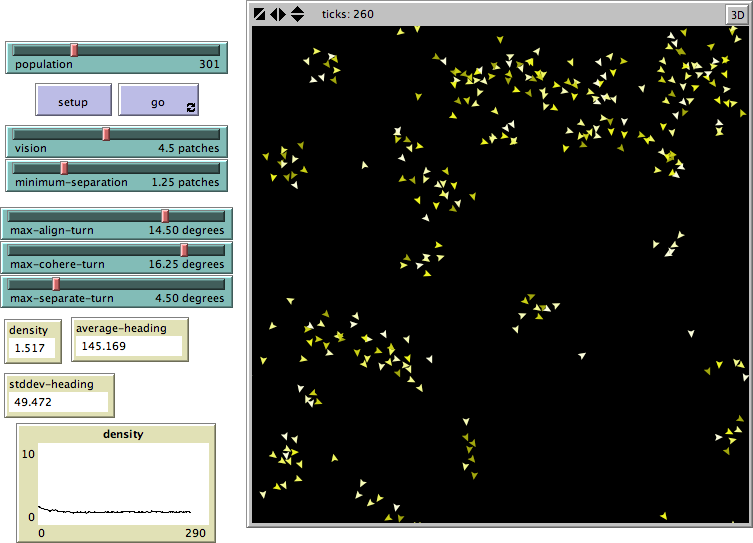
\includegraphics[scale=.5]{images/netlogoui.png}
\caption{A screenshot of NetLogo's graphical user interface while executing a flocking simulation.}
\label{fig:netlogoui}
\end{figure}

% Agent-based control parameters adjust the agent-based programs, but what is interesting is the system-level behavior [diagram]. Example.
% These system-level obvervations are typicall made by the user viewing the visualization of the world.
% Human users can generate a qualitative mapping about a world how the underlying parameters control it.
% Show example [with figures] the difference between two different systems with different qualitative system-level behaviors (boids?)
% Many emergent behaviors can be measured quantitatively to aid the user in understanding the behavior
%  This is done in netlogo with labels... as seen in figure...
Agent-level control parameters adjust the behaviors of agent-based programs.
However, scientists are not typically interested in the local interactions between agents--- they are interested in the resulting system-level behaviors that result.
For example, researchers that studied agent-based models of lane formations in army ants were interested in the traffic patterns of the lanes, not the individual behaviors of the ants \cite{couzin2003sol}.
In other work, researchers that studied locusts were interested in determining at what critical density locusts begin to swarm and destroy crops \cite{buhl2006dom}.
Typically, scientists analyze ABMs by viewing visualizations of the environment or gathering statistical data on the simulation.
For instance, NetLogo, an agent-based modeling programming environment \cite{tisue2004netlogo}, has monitors, plots and visualizations to convey system-level properties to the user.
In Figure \ref{fig:netlogoui}, monitors are displaying \textit{density}, \textit{average-heading} and \textit{stddev-heading} statistics for a flocking domain.
In addition, a plot of density shows how it has changed over time.
These tools are used by a researcher to generate a mental model of how the agent-level control parameters of the flocking domain (the sliders seen in the user interface) affect these system-level properties.

% Controlling agent-based models is: unintuitive (learning curve), /elaborate: conceptual disconnect/, example
%   user-time intensive, /elaborate: many sliders/, example
%   difficult to get a high-level view given only the agent-level parameters, /elaborate/, example
Although using ABMs for researching agent-based systems has been proven useful in a number of domains, there is a glaring conceptual disconnect from the user's perspective, between the agent-level controls and the system-level properties.
The classical ABM control method of adjusting agent-level properties is unintuitive because they only indirectly affect the system-level properties through emergence.
With the current methodology, a simulation has to be executed in order to observe what the values of the system-level properties will be.
A time consuming iterative process of guess-and-check is the only way to configure the system to have it exhibit a desired system-level behavior.
A determination of what an ABM will do at a system-level, given only the agent-level parameters, is not possible with current software.

% \fw Reduces the learning curve of the system significantly since users are dealing with a control that directly controls the system-level behavior.
% Reduces the amount of time the users physically interacts with the system because they have a reduced number of controls to deal with.
% It is easier to make qualitative determinations from a collection of system-level properties, than the values of the agent-based controls.
%   For example, give a list of agent-level controls and the resultant system-level property values... argue that the system-level property values give more information about the system.
The main goal of the \framework is to bridge the gap between agent-level parameters and system-level properties.
\fw reduces the learning curve of an agent-based model since users are interacting with the system at the system-level, instead of at the agent-level.
Qualitative analysis of an ABM's system-level properties will be a more efficient process since researchers deal with an abstraction of the system's controls.
In addition, the models learned by \fw can be inspected to gather quantitative data about the correlations between system-level properties and agent-level parameters.


\section{Wolves, Sheep and Grass}

\begin{figure}[ht]
\centering
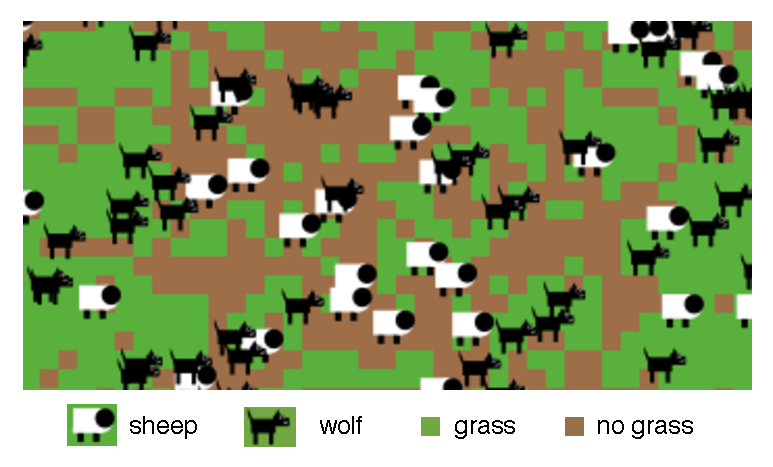
\includegraphics{images/intro_wolfsheep.pdf}
\caption{A screen shot from NetLogo's Wolf Sheep Predation model.}
\label{fig:wolfsheep}
\end{figure}




Throughout this dissertation, I will use NetLogo's Wolf Sheep Predation model \cite{wolfsheep}, which is bundled with NetLogo's standard Model Library,\footnote{http://ccl.northwestern.edu/netlogo/models/WolfSheepPredation} as an example to explain concepts.
A snapshot of its NetLogo visualization is shown in Figure \ref{fig:wolfsheep}.
This multi-agent model simulates a food chain consisting of wolf agents, sheep agents and grass in a two-dimensional space.
The model is controlled by seven agent-level control parameters, which directly affect the following agent behaviors:
\begin{itemize}
  \item The system is initialized with \textit{initial-number-sheep} sheep and \textit{initial-number-wolves} wolves.
  \item Wolves and sheep move randomly though the space.
  \item Wolves and sheep die if they run out of energy.
  \item Wolves eat sheep if they occupy the same space in the environment. Wolves gain \textit{wolf-gain-from-food} units of energy from eating sheep. The sheep dies.
  \item Sheep eat grass if they are on a location of the environment that has grass. Sheep gain \textit{sheep-gain-from-food} units of energy from eating grass. The grass dies in that grid location.
  \item Every time step, each sheep and each wolf has a chance (\textit{sheep-reproduce} and \textit{wolf-reproduce}) to reproduce asexually. Both the parent and the child split the parent's original energy evenly (i.e., parent's energy divided by two).
  \item Grass regrows after \textit{grass-regrowth-time} number of time steps.
\end{itemize}

\begin{figure}[ht]
\centering
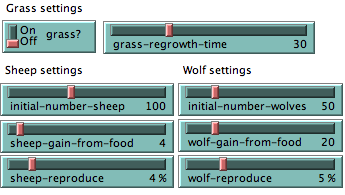
\includegraphics[scale=.66667]{images/wolfsheepcontrols.png}
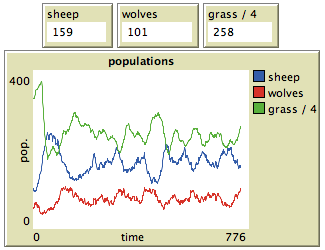
\includegraphics[scale=.66667]{images/wolfsheepmons.png}
\caption{The control and monitor interface for the Wolf Sheep Predation model.}
\label{fig:wolfsheepui}
\end{figure}

The system-level concepts we are interested in are the number of sheep, the number of wolves and the number of grid locations containing grass.
In NetLogo, these properties are displayed with monitors and a plot, as seen in Figure \ref{fig:wolfsheepui}.
The number of each population of agents may change continuously, but the average number of sheep converges.
Another interesting feature is some ecosystems fail: either sheep or both sheep and wolves go extinct.

\begin{figure}[ht]
\centering
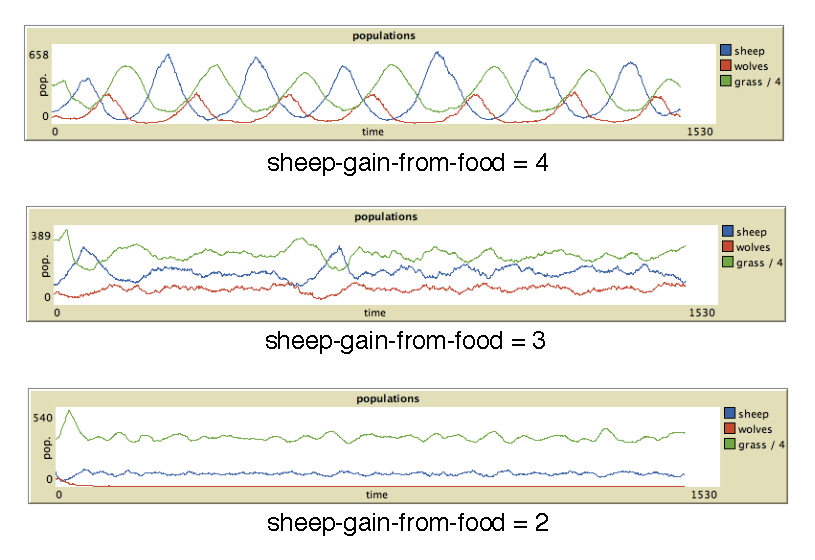
\includegraphics[scale=1]{images/different_sheep.pdf}
\caption{Differences in populations based on changes of the \textit{sheep-gain-from-food} parameter.}
\label{fig:diffsheep}
\end{figure}

After working with this ABM for some time, a user will begin to realize that changes in the control parameters will yield different types of behavior.
For example, by setting \textit{sheep-gain-from-food} to 2, 3, and then 4, major differences in system-level behavior are apparent by viewing the graphs in Figure \ref{fig:diffsheep}.
When the value of \textit{sheep-gain-from-food} is 4, the system rhythmically exhibits major changes in all three agent populations.
When the value is 2 or 3, the population remains relatively stable, but the average population values are different.
When the value is low enough (e.g., 2) the wolves go extinct.

The Wolf Sheep Predation model is a good example of the intuitive disconnect between agent-level parameters and system-level properties.
There is no clear \textit{explicit} relationship between the controls presented in the user interface and the resulting system-level properties.
An experienced user may have a qualitative understanding of the correlations, but would not be able to predict quantitative concepts, such as the average number of sheep after 2000 time steps.
In  Chapter \ref{Results}: Results, I will show that the intuitive disconnect in this domain can easily be solved by \fw.


\section{Overview of The \framework}


The foundation of this work is framing the problem of building a meta-model of an ABM as two sub-problems: the \textit{forward-mapping problem} and the \textit{reverse-mapping problem}.
In Chapter \ref{ForwardMapping}: The Forward-Mapping Problem, I will discuss how \fw maps given values of the agent-level parameters to expected system-level property values with standard regression approaches.
In Chapter \ref{ReverseMapping}: The Reverse-Mapping Problem, I will discuss how \fw maps a set of desired system-level property values to a set of agent-level parameters that would generate this behavior.
My general approach to solving the reverse-mapping problem is to interpolate configurations using the forward mapping to approximate a smooth and continuous surface.
This interpolated surface represents the space of configurations that would satisfy the system-level requirements set out by the user.
Also, in Chapter \ref{ReverseMapping}, I will discuss alternative methods for solving the revers-mapping problem.


% The framework consists of four stages: sampling, building the forward mapping, building the reverse mapping, and providing an interface to interact with the models.
% Sampling is done to generate a offline data set to use to train our regression models.
% Next, the relationship between agent-level parameters and quantitative system-level properties are developed.
% This is framed into two problems: the forward mapping problem and the reverse mapping problem.
% Finally, the framework provides standard interfaces and tools to use the two mappings to predict behavior in ABMs and control behavior in ABMs.
\fw is simple and has only a few configuration points.
This allows researchers to focus on the analysis of the system, instead of on the details of \fw.
The framework consists of three major steps: sampling, solving the forward-mapping problem and solving the reverse-mapping problem.
In these three steps, the only configurations the user must perform are: define how to measure system-level properties of interest, provide the ranges of parameters to be sampled, and plug in a regression algorithm.

I will show in Chapter \ref{Results}: Results that my framework is able to generate models of system-level behavior.
For example, \fw is able to predict the number of sheep and wolves in the Wolf Sheep Predation model, given the configuration parameter values (the forward-mapping problem).
Also, \fw is able to make suggestions for the values for the control parameters, given the the desired system-level property outcome (the reverse-mapping problem).

A more comprehensive overview of \fw is provided in Chapter \ref{Framework}: The \framework.



\section{Summary of Contributions}

% My contribution is: a \framework that alleviates the common problems in interacting with agent based models, while being domain independent, algorithm independent, and accurate.
%   an indepth look of the problem of building models of agent-based models (meta-models). How do we build them? What properties can they model? How accurately can the behavior of a ABM be predicted and controlled?
%   a learning framework that builds these models and provides users with an interface to the models.
%   I also discuss additional research topics that relate to building and using meta-models.

My main contribution presented in this dissertation is an in-depth analysis of meta-models of agent-based models.
This analysis includes a discussion of methods for using regression to build models of the correlations between agent-level parameters and system-level properties. 
In addition, this dissertation contains a survey of ways that that meta-models can be used to inspect system-level behaviors of agent-based models.

The \framework encapsulates my methodology for building meta-models of ABMs.
The implementation of \fw as software serves as a proof-of-concept to show that my approach is implementable and applicable to a variety of domains.
The software itself is a contribution, since it is available to be used by researchers interested in building meta-models of NetLogo ABMs.
The design of the general framework is a contribution as well, since it could be implemented to interact with other agent-based modeling systems similar to NetLogo, or totally independent agent-based models.


\section{Dissertation Organization}

%This dissertation is divided into nine chapters, including this one:
% Chapter Three (Related Work) provides an insight to approaches similar to \fw in motivation.
% Chapter Four (Background) is a survey of concepts in the machine learning literature and agent-based modeling literature that \fw uses.
% Chapters Five and Six define the forward and reverse mapping problems, and give an in depth analysis of how to solve them.
% Chapter Seven (Using Meta-Models) outlines useful ways to use ABM meta-models generated by \fw
% Chapter Eight (Results) surveys a number of experiments I performed to measure the effectiveness of \fw. The experiments are organized by domain, so they also serve as examples of how to apply \fw to ABMs.
% Chapter Nine (Conclusions and Future Work) summarizes this dissertation, provides additional thoughts I have regarding this work and possible directions for future work.
This dissertation is divided into nine chapters, including this one.
Chapter \ref{Framework}: The \framework explains each framework component in detail, explains how a new user would tailor \fw to a new ABM, discusses implementation details and gives an introduction to the forward- and reverse-mapping problems.
Chapter \ref{RelatedWork}: Related Work compares and contrasts approaches similar to \fw in motivation, with \fw.
Chapter \ref{Background}: Background provides information about NetLogo and regression algorithms that is useful for understanding \fw completely.
Chapters \ref{ForwardMapping} and \ref{ReverseMapping} discuss my solutions to the forward- and reverse-mapping problems.
Chapter \ref{Using}: Using Meta-Models is a survey of different ways the meta-models generated by \fw can be used to analyze system-level properties of ABMs.
Chapter \ref{Results}: Results evaluates \fw on a domain-by-domain basis and provides explicit examples of how \fw has been used.
Chapter \ref{Conclusions}: Conclusions and Future Work summarizes this dissertation, provides additional thoughts I have regarding this work and possible directions for future work.


 






\cleardoublepage

\chapter{The \FRAMEWORK}
\thispagestyle{plain}

\label{Framework}

% What does the framework do? It build meta-models that map between agent-level and system-level.
The \framework builds meta-models that map the values of agent-level control parameter values to system-level property values, and vice versa.
Learning these mappings are separate problems, which I call the \textit{forward-mapping problem} and the \textit{reverse-mapping problem}.
To solve these problems, a user of \fw ``plugs in" a regression algorithm of their choice.
The framework uses this regression algorithm to learn the mappings and then provide the user with interfaces to query them.
Once the mappings are learned, the user can query either for \textit{prediction} or for \textit{control}.
A prediction query uses the forward mapping to determine values for the expected values for system-level properties, given the system's configuration.
A control query uses the reverse mapping to suggest values for agent-level parameters, given desired values for system-level properties.
Most of the implementation details and inner workings of \fw are abstracted away from the user, who only has to attend to a limited number of configuration points.

In this chapter, I will discuss the design goals of \fw, the framework structure, software implementation details, and how well \fw conforms to the design goals.

% It frames the mapping problem into the forward mapping and the reverse mapping
% Uses a pluggable regression algorithm to solve these mapping problems

\section{Design Goals of The \framework}

% Our specific goals: provide insight and more intuitive control to agent-based models with a approach that is domain independent, algorithm independent, accurate and fast for the user.
My specific goal in designing \fw was to make the process of controlling and interacting with agent-based models more intuitive.
In addition to this central goal, \fw strives to be:
\begin{itemize}
  \item Domain independent: The design of \fw should minimize the amount of configuration that is needed for each new domain;
  \item Algorithm independent: any regression algorithm should be able to be applied with \fw;
  \item Accurate: \fw should generate accurate predictions and control suggestions; and
  \item Fast for the user -- interactions with the models generated by \fw should require minimal computational time.
\end{itemize}

% Domain independence is important because the variety in which ABMs come. We want the same general approach to work for a forest fire simulation, a boid flock or particle swarm optimization.
% Algorithm independence is important because different algorithms will model different domains better. Also, as new regression techniques are implemented in the future, they can be plugged in to increase the accuracy of \fw.
Domain independence is paramount because of the variety of ABMs.
I have designed \fw in such a way that the same general approach would work for any ABM.
Also, I strove to minimize the amount of configuration that is needed to apply \fw to a new domain.
These constraints I have set on the design make \fw broadly applicable to a number of domains, without the need for in-depth domain knowledge.
To reinforce this claim, I have tested \fw on a number of diverse domains, using the same general approach for each.

Algorithm independence in a learning framework is important because different algorithms may be more effective for modeling different agent-based models.\footnote{In general, the learning algorithms that will be discussed in this dissertation will satisfy the requirements for modeling most ABMs.
However, an in-depth analysis of which types of algorithms should be used for different classes of ABMs is outside the scope of this dissertation research.}
In addition, algorithm independence allows \fw to scale with new advances in machine learning research, since future state-of-the-art regression algorithms can be used just as easily as current approaches.

Accuracy and fast user response time appear to be obvious design goals.
However, achieving these goals require sacrifices in performance in other portions of the framework.
\fw requires a significant amount of computational time to sample different configurations of the target ABM.
These large training sets can be used to build static meta-models of ABMs that are both accurate and fast to query.
In contrast, an active learning approach would be able to learn models faster, but would require more interaction with the user, increasing the user's effort.
Likewise, optimization approaches (e.g., hill climbing) could be used to generate arbitrarily accurate results, but typically require numerous iterations and would significantly increase the response time for a user's query, because each step would have to run the ABM to calculate each fitness score, which could take several seconds.
In summary, I am making the assumption that users studying ABMs with \fw are more interested in achieving more accurate results for their research and interacting with the models quickly, than spending less time sampling.


\section{Framework Structure}

% The framework is split into three phases and four major parts.
The framework is split into several phases: sampling, solving the forward-mapping problem, solving the reverse-mapping problem, querying for prediction, and querying for control (i.e., suggesting a configuration).
Figure \ref{fig:frameworkdiag} shows how the different phases interact with one another.
Sampling makes observations from the actual ABM and then feeds the newly generated data set to the forward-mapping solver.
The result of solving the forward mapping is a function $f$, which is used to predict behavior and to develop the reverse mapping $f^{-1}$.
From an external perspective, the framework only has a limited amout of input and output:
\fw takes in observations of an agent-based model and provides interfaces to query for prediction and control.
The user queries \fw to interact with the agent-based model in an intuitive way.


Many configuration points exist, which allow users of \fw to modify the behavior of the framework.
However, the individual phases take the same output and provide the same output, regardless of the configuration.
This uniformity is what makes \fw a framework and not simply a collection of algorithms.
For example, even though different regression algorithms can be used to learn the forward mapping, the forward mapping always provides predictions of how an ABM will behave, from the user's perspective.

% Each phase feeds into the next
% Many configuration points exist in which users of \fw can change the way the framework works.
% However, no matter the configuration, the input and output of each phase is the same.

% Diagram  sampling ->  [ FM / RM ] -> usage tools






\subsection{Defining System-Level Behavior Properties}
% Measurements have to be defined to tell what to sample.
The system-level properties of an ABM must be defined by the user of \fw.
The measurement of a system-level property is a statistical or mathematical calculation based on the state of the ABM over some period of time (or ``ticks'').
% Measurements must be stable (i.e., follow the laws of large numbers); they must converge over time
The one assumption made by \fw is that the measurement is \textit{stable}, meaning that as the same configuration is sampled repeatedly, the measurement's value should vary minimally.
One way to measure stability is to calculate the standard deviation of measured values of several runs of the same system.
% Wording of the measurement is important (give the example of wolves going extinct)
The need for this assumption, ways to conform to it, and a more detailed explanation of how to define system-level properties is provided in Chapter \ref{Defining}.

For example, there are several system-level behavior properties that can be measured in the Wolf Sheep Predation model.
Three of the most obvious properties are the average number of sheep, average number of wolves, and average amount of grass over a significant number of ticks.
These are measured by individually summing the number of sheep, wolves, and grass living at each time step and dividing by the number of ticks.
Although the number of sheep and wolves change rhythmically, the average values typically converge to a single value after about 10,000 ticks.


%% HACK!! I need to physically move this around
\begin{figure}[H]
\centering
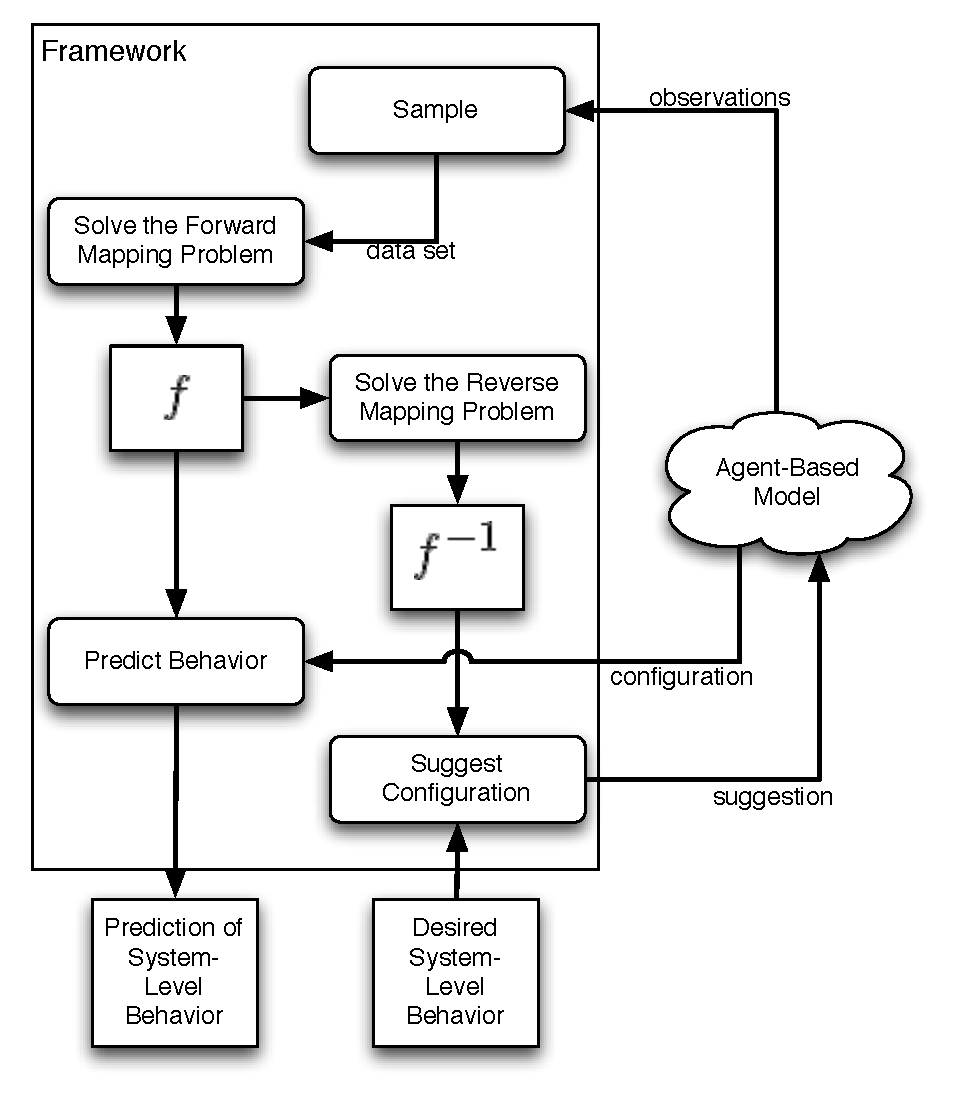
\includegraphics[scale=1]{images/framework.pdf}
\caption{An overview of the phases of \fw and how data flows among them.}
\label{fig:frameworkdiag}
\end{figure}



\subsection{Sampling}
% The first phase is sampling, in which the framework interacts with the agent-based model to generate a large enough data set for training.
The first phase is \textit{sampling}.
In this phase, numerous observations are made of different configurations of an agent-based model.
A data set is generated that contains the independent variables (the agent-level control parameter values) and the resulting system-level behaviors, for each observation.
This process can be very time-consuming, depending on several factors:
\begin{itemize}
  \item Execution time of the model -- the models will be executed numerous times, so the longer a model takes to execute, the longer the whole set of experiments will take to execute.
  \item Granularity -- more fine-grained sampling will take more time, since more points must be sampled.
  \item Dimensionality -- more agent-level control parameters result in a larger search space and naturally more points to sample.
\end{itemize}
A 120-observation sample of the NetLogo \textit{Fires} model\footnote{See Chapter \ref{Results} for detailed results.} \cite{fires} requires about thirty seconds\footnote{Most experiments are executed on a 3.0 Ghz Pentium 4 running Arch Linux.} to generate.
A large sample of 50,000 observation of a Reynolds boid flock \cite{reynolds1987} took approximately four days.

The user is required enough understanding of the domain to specify to \fw which  ranges of values should be sampled.
\fw is not able to automatically infer which value ranges are interesting, so these must be explicitly defined.

This sampling process is easily parallelizable.
Since each experiment is independent of the others, the set of all experiments can be segmented among a number of systems and processors to significantly reduce the computation time.
Once all of the experiments are completed, the results can be merged into one data set.

% For this dissertation, we either use a random sampling method or a systematic sampling method
% Future work: plug in different advanced sampling methods
For the purposes of this dissertation, I limit \fw to use a simple random sampling method (i.e., randomly select points within a specified range) or a systematic sampling method (i.e., given ranges, sample evenly spaced points).
I acknowledge that intelligent sampling strategies could improve the performance of the framework, and such strategies could be the focus future work.


\subsection{The Forward-Mapping Problem}

% The second phase is learning the forward and reverse mapping.
% This is the main focus of the learning framework.

% Explain the forward mapping problem; give an example [figure]

The \textit{forward-mapping problem} is to develop a function $f: \mathbb{R}^n \rightarrow \mathbb{R}$ that maps a provided configuration vector $\mathbf x = \{x_1, x_2, ..., x_n \}$ to several system-level behavior properties $\hat {\mathbf y}$:
\[f(\mathbf x) \rightarrow  \hat{\mathbf y}\]
The set of values $\mathbf x$ consists of all the agent-level parameters (independent variables) in the data set provided by the sampling phase.
An individual mapping is learned for each system-level behavior measurement provided by the user.
% The forward mapping is a straightforward regression problem ... Assuming this is a many-to-one relationship (due to the correct definition of the measurement)

This problem is solved with straightforward regression, such as k-nearest neighbor.
% A regression algorithm needs to be initialized with the data set (if necessary). For example, a linear regression approach would solve the least-squares problem to generate the model. Meanwhile, something like KNN has no initialization time.
In this phase of \fw, the regression algorithm is first ``initialized," if necessary.
For example, linear regression would need to solve the least-squares problem.
Meanwhile, an algorithm like k-nearest neighbor would not necessarily need to initialize anything because it scans the data set per query.
% The forward mapping problem returns an object that can be queried for configuration vector x, and returns system-level property y.
Then, the forward mapping can be used to predict values for configurations that have not been sampled.

Once this phase is completed, the user is presented with $f$, an interface to the mapping built by the regression algorithm.
The forward mapping is primarily used to \textit{predict} what the system-level property values will be, given the system's configuration.
For example, a learned mapping could be used to determine the average number of sheep given a configuration vector, without having to run the system.
Some sample predictions, given particular system configurations, are shown in Table \ref{table:ws_predictions}.
The values for a system configuration represent \textit{grass-regrowth-time}, \textit{sheep-gain-from-food}, \textit{wolf-gain-from-food}, \textit{sheep-reproduce}, and \textit{wolf-reproduce}, respectively.

\begin{table}[ht]
  \caption{Sample Predictions of Behavior in the Wolf Sheep Predation Model}
  \centering
  \begin{tabular}{c c c c}
    \hline \hline
    Configuration & Average \# Sheep & Average \# Wolves & Average \# Grass \\
    \hline
    $(30, 4, 20, 4, 5)$ & 162.8 & 76.1 & 964.8 \\
    $(30, 3, 26, 7, 5)$ & 122.8 & 90.4 & 1135.2 \\
    $(14, 3, 26, 7, 5)$ & 144.3 & 163.8 & 1621.4 \\
    $(5, 3, 17, 7, 5)$ & 946.9 & 3.4 & 1065.4 \\
    \hline
  \end{tabular}
  \label{table:ws_predictions}
\end{table}


A more in depth definition of the forward-mapping problem, specific examples of regression methods used in \fw, and the role of regression is given in Chapter \ref{ForwardMapping}.


\subsection{The Reverse-Mapping Problem}

% Explain the reverse mapping problem; give an example [figure]


The \textit{reverse-mapping problem} is to produce a mapping $ f^{-1}: \mathbb{R} \rightarrow \hat S$ from a given system-level behavior properties $\mathbf y$ to a set of
configurations $ \hat S = \{ \mathbf {\hat x} | f( \mathbf {\hat x}) = \mathbf y \}$
(i.e., $S$ is the set of behaviors that will produce behavior $\mathbf y$):
\[f^{-1}(\mathbf y) \rightarrow \hat S\]

% The reverse mapping is an "inverted" regression problem.

% We invert the forward mapping
% Inverted regression means f^-1 (building an inverted mapping)
The problem of developing the mapping $f^{-1}$ is what I call an ``inverted regression problem" and has many unique challenges.
The main challenge is that $f^{-1}$ does not, in general, describe a functional mapping:
$f^{-1}$ describes a one-to-many relationship, since $f$ is many-to-one.
Therefore, \fw cannot use standard regression techniques to solve this problem.
Instead, the default behavior of \fw is to approximate the inverse of the forward mapping, using a novel method that I developed called \textit{simplical complex inversion}.
This approach has the benefit of using the forward mapping to develop the reverse mapping, so no additional inputs from the user or additional data samples are needed.
% Elude that we will discuss our particular solutions to these problems in later chapters

The reverse mapping can be used to suggest a system configuration that will exhibit a specific set of system-level properties.
I call this process \textit{control} of the ABM, since it is controlling the ABM at the system-level by suggesting configurations.
For example, the reverse mapping could be used to suggest a configuration of $(30, 4, 20, 4, 5)$  for a desired system-level property of 162.8 average sheep (see Table \ref{table:ws_predictions}).
However, using the reverse mapping is more involved than using the forward mapping, because $f^{-1}$ returns a set of possible solutions, not a single suggestion.
If the mapping is to be used for control, any configuration in this set will satisfy the system-level requirements.
Therefore, an additional step must be taken to extract a point from the set if it is to be used to control an ABM.

The implementation details of developing reverse mappings and how to use the reverse mappings are discussed in Chapter \ref{ReverseMapping}.


% Explain how the maps are queried.
% Querying the forward mapping (example)
% Querying the reverse mapping (example)

% Possible uses: prediction and control


\subsection{Summary of Configuration Points}

% Sampling methodology
% Measurements
% Forward Mapping Algorithm
% Reverse Mapping Algorithm
The following is a summary of the configuration points discussed in this section.
For each new domain, the user must specify the following:
\begin{itemize}
   \item A list of agent-level control parameters, and the ranges within which they should be sampled.
   \item A list of system-level behavior properties and a process for measuring them.
\end{itemize}

In addition, the user may configure the following if they wish to modify the default behavior of \fw:
\begin{itemize}
   \item The sampling strategy (default: random sampling).
   \item The regression algorithm to be used for the forward mapping (defaults: k-nearest neighbor, locally weighted linear regression, or nonlinear regression).
   \item The method for the reverse mapping (default: approximate the inverse of the forward mapping).
\end{itemize}


\section{Software Implementation Details}
So far, I have discussed \fw abstractly, avoiding specific implementation details because the framework is a methodology and could be reimplemented in a number of different ways or to work with a number of different ABM simulation systems.
In this section, I discuss the details of my proof-of-concept implementation that was used to run many of the experiments documented in Chapter \ref{Results}.

% Most of the software is implemented in python, but the interaction with NetLogo is handled with Java, so that I can access the Java API.
I have tested \fw with NetLogo\footnote{More about NetLogo is discussed in more detail in Chapter \ref{Background}.} domains, however, technically any agent-based modeling system would suffice.
The rest of the framework is implemented in Python.
Each step of \fw returns its result as a file, so that it can be passed to the next step or saved for later use.
For example, the forward mapping writes the model to a file so that it can be used by both the prediction script and the reverse mapping script.

Since each domain has different variable names and nuances, the user must implement a Java program that interacts with NetLogo's API.
An abstract base class for interaction is provided to guide the development of this program.
Next, the user lists the configuration parameters and the ranges of these values so that the sampling can begin.
Measuring the system-level parameters can either be calculated within NetLogo or in Java.
For example, I modified the standard Wolf Sheep Predation model to keep track of the number of sheep at each tick.
Then, to extract the value, NetLogo's API is used to retrieve the sum of the sheep divided by the number of ticks.
A similar calculation could be performed within a Java program by retrieving each of these values individually, then performing statistics on them.
Performing the statistics calculations in Java has the benefit of not having to change the NetLogo ABM source code.


During sampling, the data set is written to a file, row by row.
Therefore, the results of several instances of the sampling, executing on different machines, can be easily concatenated.
%An example of a sampling program for Wolf Sheep predation is given in Appendix \ref{SamplingProgram}.


The regression algorithms used with \fw must conform to a standard API
%\footnote{The specification for the standard regression algorithm interface is given in Appendix \ref{RegressionInterface}.}
and are passed as arguments into the forward mapping, reverse mapping and prediction scripts.
Therefore, no configuration of these core scripts is needed, since they are ``pluggable."

An overarching ``master script," written in Python, runs all steps automatically, limiting the amount of direct interaction with the framework software.

In addition to the core framework software, I have developed a toolkit that queries the models generated by the forward- and reverse-mapping models.
The core tools include:
\begin{itemize}
   \item Query the forward mapping for a prediction by passing in a configuration,
   \item Query the reverse mapping for a set of possible solutions by passing in a desired system-level behavior configuration,
   \item Visualize the mappings.
\end{itemize}

% Give a list of agent-level variable ranges/steps
% Generate the experiments list
% Samples a NetLogo ABM with Java API, given the list of experiments, save the results
% Interact with the forward mapping regression algorithm with a python module interface
% Interact with the reverse mapping approach (discussed more in Chapter X) with a python module interface
% Different tools for selecting solutions and visualizing slices are separate python scripts.

% An overarching "master script" written in python that glues these together and automatically transitions from one to another. Each stage can be performed one by one

% More about NetLogo is covered in Background.



\section{Analysis of \fw  vs. the Design Goals}
In this section, I align the actual implementation of \fw with the design goals.

% for my reference...
%  \item Domain independent -- the design of \fw should minimize the amount of configuration for each domain,
%  \item Algorithm independent -- any regression algorithm should be able to be plugged into \fw,
%  \item Accurate -- \fw should generate accurate predictions and control suggestions,
%  \item Fast for the user -- interactions with the models generated by \fw should require minimal computational time.


% Our framework is domain independent, because it reduces the forward mapping problem to a classical regression problem of learning the correlation between the agent-level parameters and the system-level properties..
% We introduce a domain-independent approach to solve the reverse mapping problem that uses standard regression to build a space of configurations that would produce desired behavior.
\textit{Domain independence}---
My framework's implementation is domain independent, to an extent. \fw reduces the forward-mapping problem to a classical regression problem of learning the correlation between the agent-level parameters and the system-level properties.
My reverse-mapping problem solution is also domain independent because it interacts exclusively with the forward mapping, which is domain independent..
However, my implementation of \fw still requires the user to specify the agent-level parameters and how to measure the system-level properties.
This is a reasonable requirement, since automatically detecting configuration points and having a computer determine the behaviors of interest in an ABM would be a challenging unsupervised learning problem.

% Our framework is algorithm independent, because any regression algorithm (e.g., ...) can be used to develop the forward mapping and the reverse mapping
\textit{Algorithm independence}---
Any regression algorithm can be plugged into my implementation, as long as it conforms to the standard API.
A simple Python wrapper can be written to adapt an existing third-party regression algorithm to work with my implementation of \fw.
My  default process of inverted regression requires nothing special of the regression algorithm, because the inversion learning process uses the algorithm's standard forward-mapping behavior.

% Our framework is as accurate as the regression algorithms used and the data set sampled from the agent-based model. /elaborate/
% In general, I prefer spending longer sampling to generate an exhaustive data set increase accuracy and reducing user interaction delays when querying for a prediction or a suggestion for controlling.
% This shifts most of the computation time offline, instead of online, reducing user interaction time when querying the forward or reverse mappings.
\textit{Accuracy}---
No extra error is incurred by \fw itself;
the accuracy of \fw depends on the regression algorithm used and the amount of time spent sampling.
If \fw is not providing accurate results with state-of-the-art regression algorithms, either the correlations cannot be learned with current technology or not enough time has been spent sampling.


\textit{Fast for the user}---
Most computation time is spent sampling and learning the models.
These operations are offline and do not affect the response time of real-time interaction with the user.
The response time of the forward mapping and the reverse mapping are depend on the running time of the regression algorithms, but typically require less than a few seconds.






\cleardoublepage

\chapter{BACKGROUND}
\thispagestyle{plain}

\label{Background}

The purpose of this chapter is to provide necessary background information for understanding concepts related to \fw.
In contrast to Chapter \ref{RelatedWork}: Related Work, the previous research presented in this chapter do not share my motivation in \fw, but are a foundation for which \fw is built upon. 

The \framework uses preexisting research in two major areas:
agent-based modeling and regression.
The \fw is targeted at predicting and controlling behavior in an agent-based model (ABM).
The next section discusses what an ABM is, discusses some examples of ABMs, and lists some existing multi-agent software frameworks.
In the following section, I define regression, outline favorable and unfavorable properties that regression algorithms, and outline a number of regression algorithms that have been used by \fw.
Finally, I discuss methods that are used in solving the reverse-mapping problem: plane intersection and optimization.



\section{Agent-Based Modeling}

Agent-based models are implemented from the agent perspective.
Agents in ABMS are typically:
\begin{itemize}
   \item bounded by a limited global view,
   \item perform local interactions, affecting their local environment and neighboring agents,
   \item are autonomous (i.e., not following some top-down control), and
   \item may be heterogeneous (i.e., agents within the system can have different properties).
\end{itemize}\cite{epstein1999agent}
This is opposed to an ``observer" perspective, in which an overarching control system dictates what agents are to do.
For example, in NetLogo, an agent moves forward two units with the following command:
\begin{quote}
\texttt{\small > fd 2}
\end{quote}
Notice that this code is agnostic to the global direction of the agent or the position of the agent in the environment.
The code simply tells the agent to move forward two units.
In contrast, if this were to done from the observer perspective in NetLogo, the following code would be necessary:
\begin{quote}
\texttt{\small > set [xcor] of turtle 0\\
([xcor] of turtle 0 + 2 * cos([heading] of turtle 0))\\
> set [ycor] of turtle 0\\
([ycor] of turtle 0 + 2 * sin([heading] of turtle 0))}
\end{quote}
This code computes the change in the x-coordinate and the y-coordinate, given that the agent should move 2 units.
Then, it adds the result to the agent's original x- and y-coordinates.
Finally, it sets this turtle's x- and y-coordinates to the new x- and y-coordinates.
This process is cumbersome.
The agent-based property allows for a more intuitive way to build multi-agent systems.

One of the common uses of ABMs is to discover which local interactions generate a given emergent behavior of a system, through experimentation.
The research question is posed well by Epstein as the \textit{Generativist's Question}:
\begin{quote}
   How could the decentralized local interactions of heterogeneous autonomous agents generate the given regularity?
\end{quote}
To answer this question, Epstein then poses the \textit{Generativist's Experiment}:
\begin{quote}
Situate an initial population of autonomous heterogeneous agents in a relevant spatial environment; allow them to interact according to simple local rules, and thereby generate--or ``grow"--the macroscopic regularity from the bottom up. \cite{epstein1999agent}
\end{quote}
If a model accurately generates the emergent behavior of the target system, then that ABM could explain why that behavior emerges.
Agent-based models are particularly well-suited to answer the Generativist's question.

The concept of ABMs can be extended to other uses beyond modeling.
Many swarm intelligence techniques, such as particle swarm optimization \cite{kennedy1995pso} and ant colony optimization \cite{dorigo2004aco}, use a decentralized agent-based approach to solve optimization problems.
Although they are inspired by naturally occurring phenomena, their purpose is entirely separate.

Implementing systems as an ABM could be more natural than other approaches when the system cannot be defined in an aggregate manner or when individual behavior is complex \cite{bonabeau2002agent}.
ABMs are often compared to equation-based modeling (EBM), in which the model is a parametrized system of equations that describe system-level behavior (i.e., the observer perspective).
For example, a supply chain management system could be modeled as an ABM or an EBM \cite{parunak1998agent}.
In the ABM proposed by Parunak et. al, individual agents represent different companies that trade with one another.
In contrast, the EBM is a series of ordinary differential equations describing the input and output of different components of the supply network.
It is difficult to model certain behavior, such as changes in state, erratic behavior and local interactions with these observer-perspective equations.
In my example above where the agent moves forward, a relatively simple task of adjusting the position of an agent proved to be overly complicated.
When more detailed operations need to be performed, the complexity of the observer-perspective model increases drastically.
Agent-based models remedy this by simply changing the context of the programming.

% Agent-Based Models
  % Agent perspective
  % Agents follow rules, or agent programs
  % low-level interactions emerge into interesting system-level properties



\subsection{Examples of Agent-Based Models}

ABMs have been used to model a variety of different systems.
In this subsection, I outline a number of agent-based models that have been developed by other researchers in the past.

  % //Model// some real or artificial phenomena - abstract simulation - model pieces of interest
  % Uses: studying social animal behavior, studying human social interactions (traffic, disease propagation), supply chain management

\subsubsection{Reynolds Boid Flocking}

\begin{figure}[ht]
\centering
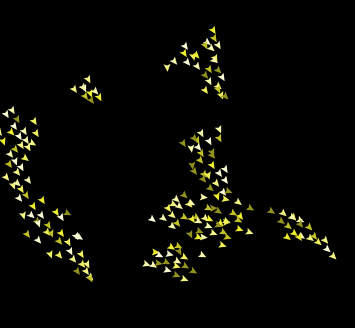
\includegraphics[scale=.66667]{images/netlogo_boidflock.png}
\caption{A boid flock moving through a two-dimensional space.}
\label{fig:netlogoboids}
\end{figure}

One of the first popular ABMs was the boid flock \cite{reynolds1987}\cite{reynolds1999sba}, in which agents move through an environment in a similar way to how birds flock.
A screen shot from NetLogo's boid implementation \cite{flocking} is shown in Figure \ref{fig:netlogoboids}.
Agents follow three simple rules:
   \begin{itemize}
      \item move away from other agents to avoid collisions,
      \item align to move in the same direction as nearby agents, and
      \item move towards the central position of local flockmates.
   \end{itemize}
These simple agent-level behaviors result in the elegant flocking behavior observed from a top-down view of the system.
This system naturally lends itself to being implemented as an agent-based model because the agents act autonomously and have local interactions with only their neighbors.
The flocking behavior is emergent and therefore would be more difficult to program directly.

Boid flocking has been used in a number of applications, such as visualizing time-varying data \cite{1382896}, clustering documents \cite{cui2006flocking}, controlling unmanned air vehicles \cite{crowther2003flocking} and art \cite{Boyd}.

\subsubsection{Social Insect Behavior}

A number of different projects have aimed at modeling insect societies.
In modeling these systems, researchers are able to gain insights into how individual agent behaviors affect their emergent behavior.
These models are typically based on observations of the real insects.

An agent-based model approach has been used to model how army ants form traffic lanes \cite{couzin2003sol}.
The particular species of army ants discussed in this work form two-way highways to reduce the amount of head-on collisions while ants are searching for food and returning food.
The authors show how the turning rates and perception of the individual ants affect the efficiency of the ants.
They found that when the turning rate is too high, ants are too willing to steer off course and intersect the path of other ants.
On the other hand, when the turning rate is too low, ants will not adjust their heading to avoid head on collisions.
By tuning their model to optimize the highway performance, they reached an accurate model of the traffic flow in army ants.
The result of this research is an accurate model that describes the individual behavior of ants in a traffic situation.

With a different species of ants, researchers were able to produce an agent-based model that simulates the process of collectively selecting a location for a nest \cite{pratt2005agent}.
This process is interesting because an entire ant colony converges on one location, even though many of the ants only have scouted one nest site.
Agents are implemented as state machines, in which agents are either exploring for a site, assessing a site, canvassing a site or committed to a site.
In each of these phases, the agent performs different actions and at any time may reject the current site and begin exploring once again.
Over time, all ants converge on a single site as a nest.
With this model, the authors showed that a colony-level decision can be made by ants following agent-based rules.

An ABM has been developed to simulate swarming locusts \cite{buhl2006dom}.
Locusts have an interesting property in that when they are isolated, they tend to not stray from their current location.
However, when locusts are accompanied by several other locusts, they begin to ``march," travelling from one area to another, consuming everything in their path.
The authors were particularly interested in determining at what density the locusts will begin to march.
By changing the number of simulated locusts in a confined space, they were able to determine at what critical density they would march.
This simulation approach is far more practical than experimenting with real locusts.
The authors suggest that their models could be used to predict when locust swarms will occur to help warn farmers to protect their crops.


\subsection{Models of Human Societies}

Although human behavior is more complicated than insect behavior, local human interactions can often be generalized to build accurate models of a subset of human society.
Most of these aim to create an accurate as possible model of the human interactions with others in order to predict some society-level behavior.

Agent-based models have been used to determine how locals would react to an incident at the Pacific Missile Range Facility (PMRF) in Hawaii \cite{zanbaka}.
The researchers used census data to represent each islander as an individual agent that either has a positive sentiment or a negative sentiment towards the missile facility.
Agents can either change its sentiment towards PMRF by either interacting with another agent that has a different sentiment or experiencing a local event.
The model simulates local events and agent interactions and displays how either positive or negative sentiment propagates throughout the island.
With this model they were able to model hypothetical situations and how they effect the sentiment on the island.

EpiSims is an agent-based simulation tool that models disease outbreaks \cite{eubank2004modelling}.
It uses estimates of how diseases are transmitted and how humans interact based on census and land-use data to realistically simulate the human society.
The system simulates individuals going to work and shopping, which exposes them to the disease and exposes the disease to others.
With this system, researchers are able to predict the effectiveness of mass and targeted vaccination strategies, given a particular community.

STREETS is an agent-based model of pedestrian traffic \cite{schelhorn1999streets}.
Pedestrian traffic is affected by two major aspects: the layout of the street network and the location of attractions.
Instead of trying to analyze the behavior of the system from this data alone, STREETS simulates people to determine a number of properties of pedestrian traffic patterns.
STREETS initializes the system with a statistically accurate distribution of individuals across the environment.
Next, the agent-based model simulates the movement of agents from their arrival point to and through the urban center.
Agents visit buildings and attractions and walk between them.
Researchers use this tool to observe a top-level view that can be used to analyze the effectiveness of the urban center layout.
Hypothetical modifications to the environment can be performed in simulation to determine if it would improve the traffic situation.



\subsection{Multi-Agent Software Frameworks}
  % To facilitate the creation of new agent-based models, many modeling environments have been developed... (give ~1 paragraph summaries of each)
Implementations of different multi-agent systems have many similarities.
To reduce the amount of ``boiler plate" code for each new multi-agent system, a number of unique multi-agent software frameworks have been developed in the past two decades.

\subsubsection{The Swarm Simulation System}
Swarm is one of the original agent-based modeling platforms, originally developed at the Santa Fe Institute in the 1990s.
Swarm is currently supported and hosted\footnote{Download Swarm at http://www.swarm.org/} by an independent organization called the Swarm Development Group
The developers' motivation was to enable researchers to focus less on implementation and more on actual experimentation \cite{minar1996swarm}.
To achieve this goal, they implemented a number of libraries in Objective-C and Java that aid in the creation of ``swarm" objects, the building block of a Swarm simulation.
The swarm objects manage the agents and handle the time schedulers that queue the order of agent actions.
Also, agents can be nested as hierarchies in swarm objects, to allow for different types of agents.
Swarm is a discrete time simulation, which means time progresses as actions occur.

Programming in Swarm can require a significant amount of programming overhead, since the libraries are not a single integrated application \cite{kleinbreve}.

    % Swarm
\subsubsection{Repast}
The Recursive Porous Agent Simulation Toolkit (Repast) is a comprehensive agent-based modeling toolkit, focusing on modeling social interactions \cite{collier2003ref}.
The toolkit is freely available to download.\footnote{Download Repast at http://repast.sourceforge.net/}
Repast is fully object oriented and attempts to be as platform independent as possible, supporting programming in Java, Python, Visual Basic.Net, and more.

Repast's features are split into six modules \cite{north2006experiences}:
\begin{enumerate}
   \item The engine module -- the core module that controls the agents, environment and scheduler,
   \item The logging module -- records execution results,
   \item The interactive run module -- manages user interaction with the model,
   \item the batch run module -- allows the user to set up a set of simulations to be ran in succession,
   \item the adaptive behaviors module -- an optional module that provides built-in adaptive agent behaviors, that use techniques such as genetic algorithms and neural networks,
   \item the domains module -- an optional module that helps define environments, such as social systems, geographic information systems, and computational game theory.
\end{enumerate}
Repast's feature set is quite comprehensive and extensible.
   
    % Repast
\subsubsection{Breve}
Breve is a unique 3D simulation environment that focuses on decentralized systems and artificial life \cite{kleinbreve}.
Like most other simulation environments, Breve is freely available.\footnote{Download Breve at http://www.spiderland.org/}
The authors of Breve tout that it aims to provide a platform for physically realistic 3D models.
The models simulate continuous time, and continuous space, unlike other toolkits which model time as discrete events and have grid world environments.
In addition, some physics such as gravity and object collision resolution with friction are built-in features of every simulation.
Breve's OpenGL display engine allow for easy to implement 3D-accelerated graphics.
Users of Breve must use a custom object-oriented language called Steve.


One of the motivating applications for building Breve was Sims' (1994) evolved 3D creatures \cite{kleinbreve}.
In this project, creatures composed of several blocks and joints compete in a game to be closest to a ball.
The features of Breve naturally fit to this domain, since it has physically realistic servos and objects that can interact with one another.
Due to these features, Breve is an interesting system for modeling individual mobile agents, as well as multiple mobile agents.



\subsubsection{MASON}
    % MASON
MASON is a multi-agent simulation toolkit developed at George Mason University and is freely available.\footnote{Download MASON at http://cs.gmu.edu/~eclab/projects/mason/}
MASON takes a different approach than previous multi-agent toolkits in that it strives to be minimalist and efficient for up to a million agents \cite{Luke}.
It is meant to be ran on a number of back-end computation servers in parallel, without visualization.
MASON does not have any domain-dependent tools or built-in environments like Breve or Repast, leaving most to the user to implement in Java.
Although MASON is quite minimalist, it is designed to be extended so that it can be used for either simple simulations or as a foundation for new simulation systems.
MASON simulations can be interacted with a separate visualization that binds to the simulation.
This is a different paradigm than other toolkits like NetLogo that are tightly coupled with the visualization.


\subsubsection{NetLogo}
    % Background information on NetLogo
NetLogo is a relatively new ABM system, which was started in 1999 out of Northwestern University as a derivative of StarLogo \cite{tisue2004netlogo}.
The software is free to download,\footnote{Download NetLogo at http://ccl.northwestern.edu/netlogo/} but not open source.
As the name suggests, the language used by NetLogo is a derivative of Logo, a Lisp-like language.
An artifact of this language that remained in NetLogo is that agents are referred to as ``turtles."

NetLogo's language is tailored to the agent-based model paradigm.
Particularly, a program can change context to an individual and execute code from its point of view.
Also, it can execute these individual actions concurrently to a population of agents.
For example, the code to ask all the agents to move forward one unit, then turn right would be:
\begin{quote}\texttt{\small ask turtles [ fd 1 rt 90 ]}\end{quote}
In addition to turtle agents, the other basic agent type is the ``patch."
Patches are organized in a grid in the two-dimensional environment that agents are confined to.
Users can interact with patches from their context, like the turtles.
Also, it is easy to retrieve turtles that are in contact with a patch and to retrieve which patch a turtle is on, from their respective contexts.
This makes turtle interactions with the environment simple to implement.

NetLogo also includes a built-in user interface and user interface editor.
The interface consists of controls, monitors and the domain visualization.
Users define controls which bind to global variables and buttons that bind to function calls.
In addition, users can add monitors and plots, which show a variable's value or plot a variable's value over time.
These are useful tools in conveying information that the domain visualization cannot.
NetLogo can be run ``headless," to facilitate parallel execution of models or to reduce run-time.

NetLogo comes with a number of extensions, most notably BehaviorSpace and HubNet.
BehaviorSpace is a tool for setting up a set of systematic experiments with different system configuration parameters.
BehaviorSpace performs a user-defined measurement value for each run and reports the result to a data set in the form of a spreadsheet.
HubNet is a server/client tool that allows several users of a system to interact with a NetLogo ABM at the same time, which is useful for classroom instruction.

NetLogo can be interacted with from an external Java API.
A NetLogo ``workspace" is instantiated as an object and can be sent NetLogo commands and can be queried for a current value.
This is useful for an number of tasks.
First, sometimes NetLogo's language is not expressive enough and some may find programming in Java more familiar.
In addition, external Java libraries (such as machine learning libraries) can be used without modification by integrating with NetLogo from its Java API.
Also, a sequential experiment system can be implemented in Java if a user would like to run experiments without BehaviorSpace.

An extensive model library with over 140 sample models are bundled with the NetLogo distribution.
These already existing models serve as excellent examples for new models as well as starting points for modified models.
Most of the domains discussed later in this dissertation are from this model library.

NetLogo is my ABM system of choice for this dissertation for a number of reasons.
First, NetLogo's learning curve is surprisingly short.
From personal experience, a new user can learn to write a domain similar to the Wolf Sheep Predation model in less than a couple hours.
In addition, the documentation\footnote{The NetLogo documentation is available at http://ccl.northwestern.edu/netlogo/docs/} is well organized and detailed.
Second, the model library provided several models that are interesting and easy to work with.
Since each of these models are implemented in NetLogo, I was able to implement a system that interacted with each of these in a similar way.
Other multi-agent system toolkits provide more flexibility in implementation, which would make identifying agent-level control parameters and system-level properties more difficult.
Third, although NetLogo's platform is well contained, the interactions possible with the Java API are superb.
I am able to implement my framework as an external modular application that interfaces with NetLogo, instead of a built-in system dependent tool.
This will make my research easily extensible to other ABM systems in the future.

  % NetLogo - used by this research
    % Concept - based off logo, 2d domain of patches, agents are ''turtles''
    % Agents are asked to perform actions from their context. e.g., ask turtles [ fd 1 ]
    % Plotting and monitors
    % BehaviorSpace extension for sampling
    % Java APIs


\section{Regression}
Regression is an integral part of this dissertation research, as it is the foundation of solving the forward- and reverse-mapping problems.
  % The reason for regression: we have independent and independent real-valued variables.
Regression techniques are used to predict values of dependent variables, given values for the dependent variables.
The typical approach is to use a model developed from a sample training set to infer new values that have not been sampled.
Also, regression can be used to smooth the natural error in sampling.

Linear regression is perhaps the simplest form of regression that fits a line to fit one independent variable with one dependent variable. It takes the form of:
\[\mathrm{y} = \mathrm{x} + b.\]
There exists a closed-form solution to determine $m$ and $b$ in order to minimize the sum of least-squares between the training data and the curve.

Unfortunately, linear regression is limited in that it only models linear relationships, and is not able to model nonlinear ones, such as rhythmic oscillations, or quadratic correlations.
Two paths are generally taken to address this concern.
The first is to use the kernel trick \cite{muller2001introduction} to map nonlinear data to be linear, but higher dimensional.
Then, once the data is projected into a space in which it is linear, linear methods (e.g., linear regression, perceptrons \cite{minsky19882perceptrons}, or support vector regression\cite{smola2004tsv}) can be used.

% Regression
   % Give definition of the regression problem
The second path are nonlinear methods, which relax the problem to learning a function $f(\cdot)$ that satisfies the following:
\[y_i = f(\mathbf x) + \varepsilon_i.\]
In this equation, $y_i$ is a dependent variable, $\mathbf x_i$ is the vector of independent variables associated with $y_i$.
Also, there is an assumption of some normally distributed and independent error with each point, denoted by $\varepsilon_i$.
The process of \textit{nonparametric} regression is to estimate this function directly \cite{fox2002r}.

Alternatively, a \textit{parametric} regression model is one in which the form of the function $f(\cdot)$ is relatively fixed.
Instead of learning $f(\cdot)$ directly, a vector of model parameters $\mathbf \beta$ are optimized to fit the data \cite{fox2002r}:
\[y_i = f(\mathbf \beta, \mathbf x) + \varepsilon_i.\]
For example, $f(\cdot)$ could model two-dimensional sinusoidal data with the model:
\[f(\mathbf \beta, (x_1, x_2)) = \beta_1 + \beta_2 \sin (x_1 - \beta_3) + \beta_4 \sin (x_2 - \beta_5)\]
Typically, the value of the sum of least-squares metric is minimized to fit the curve to the data.

  % What I need in a regression algorithm: can model nonlinear behaviors that are difficult to apply a model to and works in many dimensions; needs to build relatively smooth models for the inverted regression to be smooth.
While developing the \framework, I needed regression algorithms that satisfied a number of properties.
The regression algorithm should scale well with dimensionality, since agent-based model behavior spaces (i.e., the space of agent-level parameters and system-level properties) are typically highly dimensional.
I also needed algorithms that could model nonlinear correlations, since behavior spaces are expansive and rarely maintain linearity throughout the entire space.
However, in the ABMs I have experimented with, all spaces are very smooth locally.
That is, there is little variance in values between nearby locations in the behavior space.
Even in the situation where there is variance, the error is typically evenly distributed and cancels out if the same configuration is sampled a number of times.
Therefore, nonlinear parametric regression can fit to the overall behavior space, without having to worry about fine grained variations in the data.
Also, the mappings build by the regression models should be smooth.
This is important for the tractability of finding the reverse mapping, since bumpy surfaces will yield more intersections than smooth ones.
Therefore, regression methods that smooth the data, such as LOESS, are effective in this situation.

\textit{[\textbf{TODO}: an image showing graphs of the fires, boids, and sheep/wolf predation behavior spaces (need to make wolf/sheep data set to do this)]}

In the course of testing \fw, I used four regression techniques: k-nearest neighbor, LOESS, least-squares nonlinear regression, and Multilinear Interpolation.

  % Figure of Fires domain, boids domain, wolf/sheep predation domain behavior graphs
  % So far, I have implemented the following regression algorithms to work with \fw: K-Nearest Neighbor, LOESS (Locally weighted scatterplot smoothing, least-squares Non-Linear Regression, Multilinear Interpolation
\subsection{K-Nearest Neighbor Regression}
  % K-Nearest Neighbor Regression
    % Concept - Take k-nearest neighbors and average them
K-nearest neighbor (KNN), in general is the process of selecting the $k$ nearest points to some point $\mathbf x$.
These points can then be used for classification or regression.
In the simplest case, each neighbor's $y$ value is averaged to inter a value $y'$ for the given point $\mathbf x$.
KNN is easy to implement and accurate with large data sets.
Accuracy of this regression can be improved by weighting points by distance or by using a secondary regression algorithm (e.g., linear regression) on the neighbors.

    % The role of KNN - easy to implement, accurate with large data sets
We use KNN in our results as a baseline, since it is easy to implemente and accurate with large data sets.
In addition, it is nonparametric, which makes it agnostic the the shape of the behavior space.
This results in KNN requiring no configuration or tailoring to a particular domain.

    % Slow with large data sets because of all the distance calculations needed.
      % Can be sped up with advanced nearest neighbor search, such as a kd-tree or local sensitivity hashing.
However, when implemented naively, the run-time scales linearly with the size of the data set because the process of finding the nearest neighbors requires a scan of all data points.
This search time can be reduced with the implementation of faster searching techniques, such as locality sensitive hashing \cite{gionis1999similarity}, among other methods.
Even with faster neighbor locating techniques, some sort of search is required for each query to KNN.

The spaces generated by KNN are not continuous (particularly if the neighbors are not weighted).
This is because similar points will have the same neighbors and, in effect, have the same predicted value.
There are separations in which on one side the k-nearest neighbors will include a particular data point, meanwhile on the other side it will not.
At this separation, a noncontinuous jump will occur in predicted values.
This can be a problem for solving the reverse-mapping problem because the intersection between hyperplanes generated by KNN will not intersect smoothly.
This can be remedied by using KNN in conjunction with multilinear interpolation.
      
\subsection{Robust Locally Weighted Regression and Smoothing Scatterplots (LOESS)}


    % Advantages: nonparametric (useful for my domains), 
    % Role in \fw : accurate and nonparametric. Conceptually, if we sample infinitely with LOESS, we will get a very smooth graph (which makes it nice for inverted regression).
Robust Locally Weighted Regression and Smoothing Scatterplots (LOESS) is a mature nonparametric regression technique for fitting curves to data   \cite{cleveland1979robust}\cite{cleveland1988locally}.
Similar to k-nearest neighbor, LOESS uses local points to infer values of data points.
LOESS also iteratively smooths the regression curve, allowing for variable magnitudes of smoothing.
This is important for particularly noisy data sets.
The role of LOESS in the testing of \fw is it is more robust than KNN, yet still nonparametric.

    % Concept - take some subset of neighbors, weight them, and then perform linear regression on them
Abstractly, LOESS fits a new $\hat y_i$ to every $\mathbf x_i$ to replace the original noisy $y_i$.
Then, LOESS iteratively smooths each $\hat y_i$ to reduce variability.
Specifically, LOESS follows the following steps:
\begin{enumerate}
   \item Initialization step -- for each $\mathbf x_i$, weight all other points $x_j$, where $j = 1...n$, based on a weighting function $W(\mathbf x_i, \mathbf x_j)$. $W$ weights closer points higher. Perform weighted linear regression to infer $\hat y_i$.
   \item Smoothing step -- For each $\mathbf x_i$, weight all other points based on $w_i$, as well as a new weight function $\delta$, which returns magnitude inversely proportional to $y_i - \hat y_i$ (i.e., the larger the distance, the lesser the weight). Perform weighted linear regression to infer $\hat y_i'$.
   \item Set each $\hat y_i$ to $\hat y_i'$.
   \item Repeat the the smoothing step as many times as necessary.
\end{enumerate}
Values in between $\mathbf x$s can be now be interpolated.

    % Role of the smoothing parameter -- how much data is used to fit each polynomial
LOESS can be customized in a number of ways.
The different weighting functions can be changed to change the amount of influence other points give to the linear regression step.
Typically, these weighting functions have a ``smoothing" parameter, when increases the influence of further away points, effectively reducing the strong influence of local points.
Adjusting the smoothing parameter is important because if it is too low, the regression curve will be erratic, meanwhile, if the smoothing parameter is too high, some features of the curve may be eliminated.

  % LOESS
    % Weight function weights points by distance -- most common function is the tri-cube function
LOESS is relatively computationally expensive in comparison to other approaches.
This is because more weights are applied and points are readjusted iteratively a number of times.
However, the model can be built offline and then stored.
Once the $\hat y_i$ values are inferred, they can be used to interpolate new points (similar to multilinear regression) in response to queries.
This provides a quick response time to users wanting to infer to $\hat y$ values.
This fits one of the design criteria of \fw: the regression algorithm should be fast for the user.

The \textit{R} statistical package\footnote{R website: http://www.r-project.org/} has a built in LOESS function.

\subsection{Nonlinear Regression}
\cite{gallant1975nonlinear}
  % NonLinear Regression
    % Concept - take a model of the data, optimize the parameters to minimize least squares.
    % Accuracy is largely dependent on the model
    % Limited (for example, had trouble modeling the simple sigmoid looking thing from the fires domain).
    % Advantage: fast to query
    % Role in \fw: algebraically invertible (more in chapter: reverse mapping)

\subsection{Multilinear Interpolation}

  % Multilinear Interpolation
    % Concept - given corner points of a hypercube (knots), interpolate some point inside of it with linear interpolation; interpolate dimension my dimension until the point is reached.
Multilinear interpolation is a dynamic approach that uses multi-dimensional interpolation between ``knots" to generate a smooth surface across a space of any dimension \cite{davies1997multidimensional}.
Knots are sampled data points, scattered across the behavior space in a regular fashion such that the knots, when connected, form hypercubes.
When a point $\mathbf x$ is queried, multidimensional interpolation is performed using the corners of the hypercube to infer the value of $\hat y$.

    % Downside - sampling needs to be systematic: remedy- use another regression algorithm to build the knots. This has the benefit of being faster than other approaches (the interpolation is fast, the regression may be slow, and the knots can be built ahead of time)
The major downside to multilinear interpolation is that the sampling needs to be systematic and even spaced.
To remedy this situation, another regression algorithm is used to compile a set of evenly spaced points.
These evenly spaced inferred points area then passed to a traditional multilinear interpolation approach.

In this dissertation, I typically use multilinear interpolation as a supplement to the other regression approaches.
A number of points can be inferred with another regression algorithm and then interpolated between with this approach.

    % Faster than some of its counterparts
    % builds smooth mappings of multi-dimensional spaces

\section{Inverting Regression}
% How does inverting regression fit into \fw? We invert the forward mapping to solve the reverse-mapping problem.
% Our two major approaches to this are optimization and plane intersection.
% More approaches are possible and are discussed in Chapter X: The Reverse-Mapping problem, but require limited amount of background information.


\subsection{Plane Intersection}
   \cite{patrikalakis1993surface}
    % Plane Intersection
       % What does plane intersection do? it takes two hyperplanes and returns the intersection.
       % Iterative divide and conquer method (printout on my desk)

   % How we use plane intersection: The solution to the reverse-mapping problem is the intersection of the forward mapping and the plane representing the desired behavior.
   % Give example
   % Figure example

   % Benefits of this approach: gives a space that represents the intersection, instead of just one point.
   % Slow

\subsection{Optimization}
    % Optimization
       % Minimize the distance from the result of the forward mapping to the actual result
       % Stochastic Hill Climbing
           % very simple, works well in domains with not many local minima
       % Other possible approaches:
           % Gradient ascent, genetic algorithms

   % How we use optimization: Try to minimize the distance between the produced system-level property and the desired system-level property by adjusting the agent-level parameters.

   % Benefits: fast
   % bad: only finds one solution


\cleardoublepage

\chapter{DEFINING SYSTEM-LEVEL PROPERTIES}
\thispagestyle{plain}

\label{Defining}

% Definition of a system-level property
System-level properties play a central role in this dissertation.
A system-level property is a mathematical measurement of some non-explicit concept of interest in an agent-based model.
These properties are typically non-explicit, and dependent in complex ways on the explicit parameters, which means that inferring their values from just the given agent-level configuration parameters is difficult.

% Discuss how system-level properties are identified
% Discuss how system-level properties are mathematically defined
Identifying which system-level properties of an ABM to analyze is the first step of using the \framework.
Deciding which features should be measured is a task for the user of the framework and will be influenced by what that user finds interesting or what that user needs to analyze.
Each system-level parameter is defined as a mathematical measurement of the behavior in terms of observable features of the ABM.
For example, the average number of sheep in the Wolf Sheep Predation model is a system-level property of the system that is calculated by averaging the number of sheep measured in each time step over the lifetime of the system.
The framework utilizes the user-provided mathematical definition to create a data set that is used in the forward mapping.

% Give an outline of the chapter
In this chapter, I discuss the problem of defining system-level properties for use in \fw.
First, the important ``stability assumption" and the consequences of this assumption are explained.
Next, a comprehensive list of common system-level property classes is outlined.
This list should be useful for users of \fw in defining their own system-level properties.
Then, the process in which \fw uses to sample an ABM is explained.
Finally, software implementation details are given for this particular step of \fw.


\section{The Stability Assumption}

% Before delving into the topic of defining system-level properties, I first discuss this assumption
Before delving into the topic of defining system-level properties, I first discuss the ``stability assumption."
Understanding this assumption and its consequences is important in defining system-level properties so that they will be measured accurately by \fw.

% A measurement of a system-level property should be stable.
% Explain what stable means
%  the sampling error is normally distributed 
% For example, the percentage of trees burned down
\fw assumes that the naturally occurring error for sampled values of a system-level property must have the following feature: the expected mean and expected median of the behaviors should be approximately the same.
In other words, the errors should be expected to be evenly distributed around some value $\bar y$, in  both magnitude and quantity.
Errors following a normal distribution will have this property.
For example, the percentage of trees burned down in the Fires\footnote{The Fires model is discussed in more detail in Section \ref{sec:Fires}.} model will vary from run to run, but for the most part will be centered around one value for a particular configuration.

% Explain the need for stability - we are trying to develop a functional mapping to solve the forward-mapping problem. Without this assumption, we cannot use regression(see background).
If this assumption does not hold, regression algorithms will bias their predictions.
As more points are sampled, the regression algorithm's predictions will converge on the value provided by the mean of measured values.
However, the median may be a better predictor of the expected behavior if the errors are not normally distributed.
This problem is best explained with an example.


% This is an example explaining the need for stability
In the Wolf Sheep Predation domain, a simple system-level measurement is the average number of wolves after a thousand time steps.
This number can be misleading, because certain configurations will \textit{sometimes} result in the wolves going extinct (i.e., zero wolves).
Other times, the same configurations will result in the wolves converging to a stable non-zero population.
When the wolf population does stabilize, it generally converges upon the same population value, $\bar w$.
However, the average of successive runs will result in a bimodal distribution, with a single spike at zero and a tight distribution of values around this stable population size, as shown in Figure \ref{fig:num_wolves}.
Unfortunately, this average is not useful in any way, since it does not tell how often the wolves will go extinct or what their population will be, should it be the case that the population stabilizes.

%% Have a figure here that shows a histogram of wolf populations given the same configuration.
%% It will show a large number of wolf populations at zero and then a bell-curve like structure near the true value.
%% Show the median and the mean

To remedy this problem, the population measure can be decomposed into two components: the average populations in the case where the wolves become extinct and in the case when they do not.
The average number of wolves $\bar w$ can be then be posed as:
\[\bar w = \mathrm{P}(extinct) * (\bar w | extinct) + (1 - \mathrm{P}(extinct)) * (\bar w | \neg extinct) \]
where $extinct$ is true when the wolves became extinct, $\mathrm{P}(extinct)$ is the probability that the wolves become extinct, and $(\bar w | \neg extinct)$ is the average number of wolves, given that they do not become extinct.
The value of $(\bar w | extinct)$ is zero, so the left-hand side of the above equation is zero.
Therefore, the equation can be simplified to:
\[\bar w = (1 - \mathrm{P}(extinct)) * (\bar w | \neg extinct) \]

As stated earlier, $\bar w$ is biased because in some cases an experiment will return zero and sometimes it will return $(\bar w | \neg extinct)$.
However, the values $\mathrm{P}(extinct)$ and $(\bar  w | \neg extinct)$ are useful in describing the system's behavior and are more stable (and accurate) than just using $\bar w$.
The system-level properties that should be measured for the Wolf Sheep Predation model are not the average number of wolves, but the average number of wolves given that they did not go extinct, and the probability of the wolves going extinct.

To calculate the value of $\mathrm{P}(extinct)$, one can divide the number of samples that exhibited zero wolves by the number of total samples for that configuration.
To calculate the value of $(\bar w | \neg extinct)$, one can average the population size of the wolves in the samples in which they did not go extinct.

The histogram in Figure \ref{fig:num_wolves} illustrates why $\bar w$ is a poor metric for this domain.
I measured the average number of wolves post-convergence in 850 runs of the same configuration\footnote{The parameters were grass-regrowth-time = 22, initial-number-sheep = 100, initial-number-wolves = 50, \\
sheep-gain-from-food = 4.7, wolf-gain-from-food = 20, sheep-reproduce = 3\%, wolf-reproduce = 4\%. } of the Wolf Sheep Predation model.
In this experiment, 303 of the 850 samples resulted in the wolves going extinct.
The other 547 samples had their wolf populations stabilize.
The average number of wolves over all samples $\bar w$ is 44.69.
The value 44.69 has little meaning in this domain, since it does not tell us about the stable wolf population size, or how often the system will exhibit zero wolves.
In fact, the actual number of wolves is \textit{never} close to $\bar w$.
The estimated probability of extinction is $P(extinct) \approx 303 / 850 \approx .356$.
The average number of wolves in a stable population is $(\bar w | \neg extinct) = \sum (w_i) / 547 \approx 69.45$.
These two values explain the the behavior of this particular Wolf Sheep Predation model instance more accurately than $\bar w$.

\begin{figure}[ht]
\centering
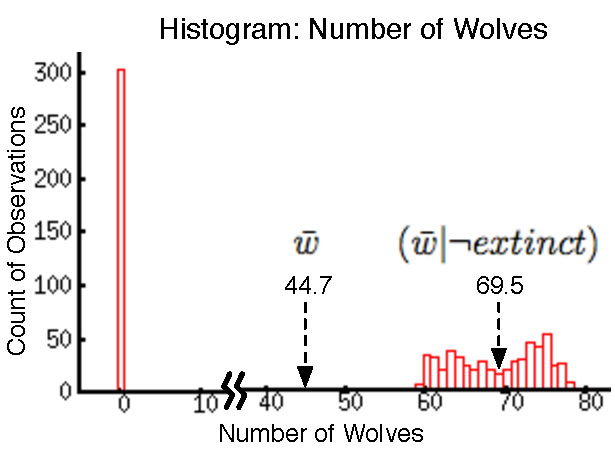
\includegraphics{images/num_wolves.pdf}
\caption{A histogram of the number of wolves after many successive runs shows that the average number of wolves is a poor measure of the system behavior.}
\label{fig:num_wolves}
\end{figure}


% In most situations, a nonstable measurement could be the result of two situations: there is an underlying threshold effect or biased readings before convergence.
In many situations, non-stable system-level properties are the result of some sort of \textit{threshold effect}.
Threshold effects are sudden changes in behavior, given a small change in the configuration.
Threshold effects are also sometimes referred to as \textit{tipping points}.
In ABMs that incorporate random behavior, configurations that are on a boundary of a threshold effect can exhibit erratic behavior, as in the Wolf Sheep Predation example.
Typically, this problem can be overcome by decomposing the property into several sub-properties that describe the threshold effect. 
This approach provides useful and accurate information in the Wolf Sheep Predation example.

\section{Common Classes of System-Level Properties}

% Many system-level properties can fit into a certain category
Through the course of identifying a number of system-level properties in a variety of domains, I have found that most properties fit into one of these general classes.


\subsection{Average of a Value}
% average value over the life of a system
One of the simplest measurements is the average value of a property over the life of the system, which is useful for measuring behavior that converges over time.
To measure this property, the property is measured every at time step until a predetermined stopping point, and then averaged.

\begin{figure}[ht]
\centering
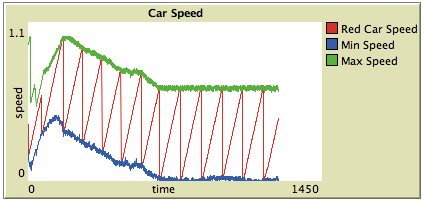
\includegraphics[scale=.75]{images/traffic_converge.png}
\caption{The behavior of the NetLogo Traffic Basic ABM converging after about 650 time steps.}
\label{fig:traffic_converge}
\end{figure}


A few modifications to this simple approach are possible.
First, the recording of values can be delayed for a number of time steps to allow the system to converge.
If convergence is ignored, the values recorded before convergence may bias the results in an unexpected way.
To remedy this, only the points post-convergence are used for the average.
The next step is to determine when this ``post-convergence" happens.
The simplest method is to determine a duration of timeaftern which the model will usually have converged.
Another naive method is to just sample for a very long time.
As time passes, the average will converge to the convergent value, since more values representing the convergent behavior will factor into the average.
A more advanced technique would be to detect when the system values have stopped changing significantly and start measuring at that point.

In Figure \ref{fig:traffic_converge} (a plot from the NetLogo Traffic Basic ABM), the maximum and minimum speeds of the vehicles converge to .65 and 0, respectively.
However, before time step 650, the behavior was quite different than the eventual convergent behavior.
If each time step (0 to 1250) were averaged, the maximum speed value would be biased to be larger than .65.
This number has some meaning, but not the ``average top speed" that was expected.
The average should be comprised of values after time step 650 to match the actual measurement with the expectations.

This class of measurement should not be used on properties that diverge (i.e., fail to converge on a single value over time).
In divergent cases, the average will continue to increase or decrease as more time steps are used in the measurement.
Instead, the average value should converge as more time steps are measured.
The values produced by the forward and reverse mappings will be inaccurate and meaningless if this property does not hold because the value would be dependent on how many time steps the system was sampled, and would have very little to do with the value of the behavior itself.

\subsection{Variance of a Value}
% variance of a value over the life of a system
The variance of a value over the life of a system is a useful metric for determining how ``stable" the property is.
If the property changes significantly from one time step to another, the variance will be higher than that of a property in which the value remains stable.
Figure \ref{fig:variance_compare} shows a comparison between two situations in which the variance of values are different.

\begin{figure}[ht]
\centering
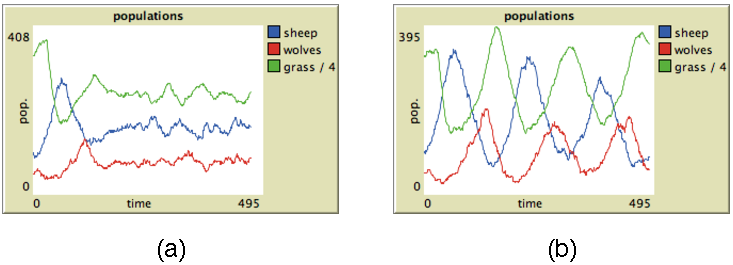
\includegraphics{images/variance_comparison.pdf}
\caption{Two different behaviors in the NetLogo Wolf Sheep Predation ABM with similar average sheep, wolves, and grass values. The two can be distinguished by the variance: the values in (a) have a lower variance than the ones in (b).}
\label{fig:variance_compare}
\end{figure}

Similar to averaging system-level properties over time, only values after convergence should be used to calculate the variance.
This must be done to avoid biasing the variance of the behavior after it has converged.
Taking this problem into consideration is important for the variance metric because systems' behaviors typically vary significantly before convergence.

Also similar to the average value metric, this variance metric should not be used on behaviors that diverge.
As a divergent property value continues to increase or decrease, the variance will increase.
The variance converges on a single value as more time steps are sampled, for the same reasons that the average metric should converge.


\subsection{Probability of a Threshold Effect}
% probability of an event occurring in the system
Threshold effects are binary properties that may or may not appear in a run of a system.
These tipping points divide the behavior space into configurations that exhibit the threshold effect and ones that do not.
Configurations near the threshold will often vary in which behavior side of the threshold they will converge to.
For example, in the Wolf Sheep Predation ABM, wolves may or may not be extinct when the system converges.
With some configurations, the wolves will always go extinct, but in others the wolves never go extinct.
Configurations on the boundary between wolves going extinct and not will exhibit both of these outcomes in different runs, due to the inherent randomness in the system.

One particularly useful metric for analyzing threshold effects is the probability that a certain configuration will exhibit the threshold effect.
For example, in the Wolf Sheep Predation ABM, a system-level property could represent the probability that the configuration will result in the wolves going extinct.
To measure this property, several experiments need to be executed for a single configuration. 
The probability is estimated by calculating the proportion of iterations that had no wolves, to the total number of experiments.
The value of this probability should converge as more experiments for a single configuration are executed.




\subsection{Measuring a Value That Changes Over Time}
The previous measurements assume that the behavior will converge over time, which is not the case for all behaviors.
Also, there are situations in which the average value or the variance of a value does not convey enough information.
% There are a number of properties that change over time  want to be measured
In particular, properties that change over time may not fit into the above classes.

% So far, all properties have had scalar values,
So far, all properties have been scalar values.
The framework works only with scalar values and is unable to naturally predict how a behavior will change over time.
% therefore, it may seem that it is impossible to measure behaviors over time, since these properties change.
% With a change of perspective, this is possible.
% to measure a system-level behavior that changes over time, the system-level properties used by \fw are scalars that represent this behavior in a parametric model.
To circumvent this issue, the system-level properties can be parameters of a parametric model that represents a behavior that changes over time.
Predicting each behavior is essentially a nonlinear regression problem, in which the independent variable is time and the dependent variable is the property.

% The parameters are the system-level properties are learned in the forward mapping process and can be used to predict the parameters of the model.
The parameters of the behavior's parametric model are learned in the forward mapping process as individual prediction problems: $N$ different forward mappings will be learned, one for each of the $N$ parameters.
The value for each parameter is predicted by the corresponding mapping, given the system's agent-level configuration.
These predicted parameters can be plugged into the parametric model to generate a curve that represents the behavior over time.

\begin{figure}[ht]
\centering
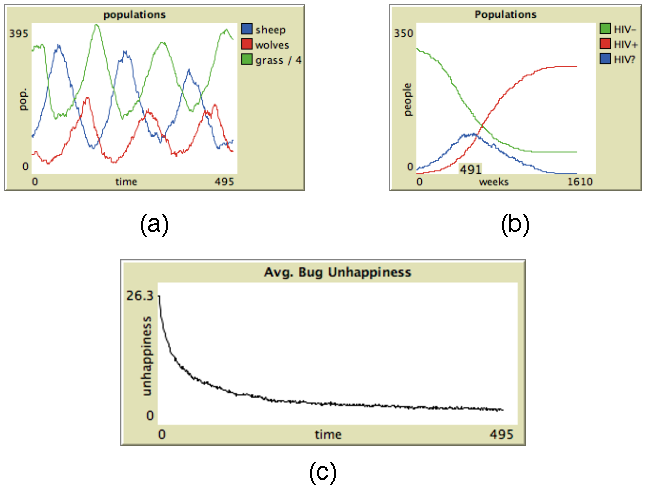
\includegraphics{images/overtime_compare.pdf}
\caption{Different types of behaviors that change over time in NetLogo ABMs. }
\label{fig:overtime_compare}
\end{figure}


This approach can be applied to a number of phenomena, such as the ones illustrated in Figure \ref{fig:overtime_compare}.
In Figure \ref{fig:overtime_compare}(a), the animal populations in the Wolf Sheep Predation model vary rhythmically and could be modeled with sine curves.
The parameters of these behaviors modify the magnitude, height, and frequency of the sine curves.
In Figure \ref{fig:overtime_compare}(b) (a plot from the NetLogo AIDS model \cite{aids}), the \textit{HIV-} (people without HIV) curve decreases and  \textit{HIV+} increases in a sigmoid pattern.
The parameters of these two sigmoid behaviors modify the shape of the sigmoid function.
The \textit{HIV?} (people who have HIV but do not know it) value appears to follow a curve that is similar to a probability distribution. 
However, it is simpler to model this property in terms of the other two: the HIV- and HIV+ values subtracted from the total population.
In Figure \ref{fig:overtime_compare}(c) (a plot from the NetLogo Firebugs model \cite{bugs}), the behavior converges to zero over time.
The rate of convergence (i.e., the slope of the curve) would be the parameter for the model of this behavior.
This general approach is applicable to any property that can be described by a parametric regression model.

These system parameters are measured during sampling by performing parametric nonlinear regression for each experiment
to determine good values of the parameters.
These parameters are the system-level properties for \fw, but can be interpreted by the user as the parameters to the regression model.

Custom models can be developed for particular domains.
Consider the NetLogo Traffic Simple simulation, in which cars move in a single lane.
Traffic jams appear in waves, which is illustrated by the speed of the red car,\footnote{Nothing is special about the red car in the Traffic Simple situation. It is singled out to show the traffic pattern from the perspective of an individual.} as illustrated in Figure \ref{fig:traffic_converge}.
We would like to develop a mapping to represent the velocity of the red car.
From visual observation, it appears that the red car has a constant minimum speed and a maximum speed.
It is known that the acceleration is linear from the programming of the model.
Also, the red car follows a rhythmic behavior: the car reaches a certain speed, then stops.
With these observations, the information necessary create a wave-like parametric model that describes this behavior is available.
 The following variables are used in the parametric wave model:
\begin{itemize}
  \item Let $A$ be the amplitude of the wave (i.e., the maximum velocity minus the minimum velocity).
  \item Let $T$ be the period of the wave (i.e., the time between the occurrence of a maximum velocity and the occurrence of a minimum velocity).
  \item Let $h$ be the height of the wave (i.e., the minimum speed).
\end{itemize}
The behavior within each period is linear, so it can be described as a simple linear model:
   \[speed(t) = \displaystyle \frac{A}{T} ~{} t + h.\]
Since this behavior is periodic, modulus $T$ is used to reset the behavior back to the minimum spread:
   \[speed(t) = \displaystyle \frac{A}{T} ~{} (t~{}\mathrm{mod}~{} T) + h. \]
The forward-mapping problem would involve predicting values for $A, T,$ and $h$, given the configuration of the system.
For each experiment, nonlinear regression is used to find good values for $A, T,$ and $h$, which are recorded as the dependent variables.



\section{Sampling}
The sampling process may begin once the system-level properties are defined.
% Two major steps:
%  1. Retrieve raw data from the simulation
%  2. Compute on that data to generate the properties of interest
The \fw sampling process consists of two major steps:
(1) retrieve raw data (i.e., observed agent behaviors at each time step) from the simulation; and (2) use that data to compute the values of the system-level properties (e.g., average and variance of specific behaviors).
Instead of performing the calculations while sampling, I prefer a method of computing the actual statistics from a raw data set.
This process permits new statistics to be measured using the raw data at a later point in time without having to re-sample the system.

% \fw typically uses a evenly distributed random sampling technique.
The \fw uses an evenly distributed random sampling technique.
Ranges for parameters are passed to the sampling program and random values within these ranges are generated for each experimental configuration.
%  this is useful for changing the size of the dataset dynamically
This technique is flexible because it allows the size of the data set to be changed dynamically for testing purposes.
Also, new points can be sampled to increase the accuracy of the data set in a particular area.
The regression algorithms used with \fw assume randomly distributed data.
% More advanced sampling techniques could be used in the future.
More advanced sampling techniques could be used in future work.

% Sometimes... Discuss the need for doing several runs on the same configuration
Sampling the same point repeatedly, instead of generating a new point per experiment, has several uses.
Different samplings of the same point could be used to:
\begin{itemize}
   \item Measure the variance of a variable between samples to determine its stability,
   \item Determine the probability of a threshold effect being exhibited,
   \item Smooth the data set by reducing natural error, or
   \item Generate more accurate individual points.
\end{itemize}
For these reasons, I typically sample each randomly selected point several times, instead of sampling a wider variety of points once.
% Discuss the selection of number of steps the ABM should run

\section{Implementation Details}

The \fw implementation for defining system-level properties and performing sampling is designed to require a minimal amount of user programming.
The sampling process consists of four distinct steps:
\begin{enumerate}
% Steps:
%  1. identify what properties are needed in the simulation and the ranges of values we want to configure --- that are needed to perform the system-level properties
\item Identify, by name, which NetLogo properties need to be extracted from the simulation in order to calculate the system-level properties, and specify how often (i.e., time steps passed) each property should be measured.
\item Specify all ABM configuration parameters by name, along with the minimum and maximum values that random configurations will lie within.
%  2. Sample the ABM to generate a raw data set
\item Run the sampling application to generate the raw data set.
%  3. Pass the raw data set through a script that converts the raw entries into the desired system-level properties to create a new data set
\item Pass the raw data set through the map\footnote{The name ``map" is to signify similarity to LISP's map function.} program, which converts the raw entries into a more compact data set that contains the desired system-level behaviors and relevant configuration parameters.
\end{enumerate}

% First step: the sampling program is written in java
%  the sampling program is given the ranges that are to be sampled,
%  and the data values that are needed
The sampling program is written in Java so that it can interface with NetLogo's Java API, which is used to run the ABMs.
All of the user-provided information is passed to this program in a text configuration file.
A program that generates values in an identical format to the default sampling program could replace the default sampling program.
Replacing the default sampling program would be useful for taking more control of the sampling process; for instance, to implement an advanced sampling strategy.

% The second step: the sampling program performs the sampling
The sampling program prints the raw data to the standard output (stdout).
The data is tab-delimited to separate items within entries; each entry is delimited by a newline.
%  the raw data is returned to standard out. The data is tab delimited to separate items within entries. Entries are delimited by newlines.
The entries are recorded in the order specified in the configuration file, so the configuration file can be used to give each column an identifiable name.
%  The output file could be redirected to a file to be stored for future use, if necessary
The standard output could be redirected to store data in a file or piped to the next step.


% The third step: use the ``map" script to parse the raw data, and output a data set that contains the system-level properties.
In the final step of sampling, the ``map" Python program is used to parse the raw data and output a data set that contains the system-level properties.
%  the map script parses the data for each entry.
The map script parses the data for each entry and returns aggregate or expanded statistics, per row.
The output of the map function is then passed to the forward-mapping problem solver, which is covered in the next chapter.

%    the parse returned is a hash table object where the keys are the names of the raw data items and the values are the values inside, as strings.
%The parse returns a hash table object (Python dictionary) per entry, in which the keys are the names of the raw data items and the keys are the values, represented as a string.
%  the map script is passed a user-created python module that is used to compute the values of the system-level properties, from the raw data.
%The map script is passed a user-created Python module that is used to compute the values of the system-level properties from the raw data.
%  this user-created python module has a list of functions that each returns a value for a system-level property.
%This user-created Python module contains a list of functions that each returns a value for a different system-level property.
%  map returns a new data set to standard out, containing the configuration parameters and the system-level properties.
%Map returns new data sets to individual files (one per system-level property), containing the configuration parameters and the system-level property.
%  simple example
%  list example
%  More details on how to create this python module is covered in Appendix XX.
%More details on how to create this Python module is covered in Appendix \textit{[TODO]}.
%The name ``map" was chosen because it is a similar process to functional programming's \textit{map} function.









\cleardoublepage

\chapter{APPLICATION DOMAINS}
\thispagestyle{plain}

\label{Domains}


Four target domains are used to demonstrate \fw in action, which show the effectiveness of \fw in a variety of different types of situations.
In Chapter \ref{Results}: Results, experiments are performed on each of these ABMs to evaluate \fw.
No modifications to \fw have to be performed to have \fw compatible with these domains, which shows that \fw is domain independent.
In each of the domains enumerated in this chapter, I give a brief overview of what the ABM represents, what configuration parameters are available, and what system-level properties I have defined.

\section{NetLogo Fires}\label{sec:Fires}

\begin{figure}[ht]
\centering
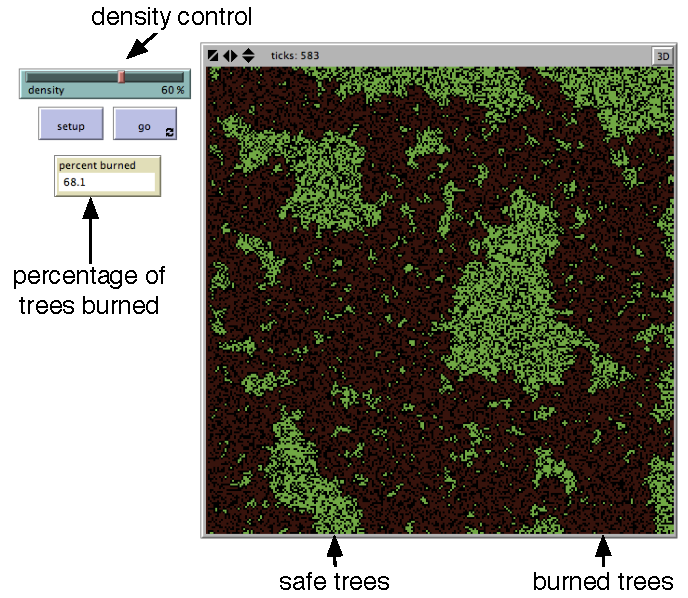
\includegraphics[scale=1]{images/fires_ui.pdf}
\caption{Screen capture of the Fires NetLogo ABM.}
\label{fig:firesui}
\end{figure}

The NetLogo Fires ABM is the simplest ABM tested in this dissertation.
In this ABM, trees are distributed throughout a $250 \times 250$ grid world.
A fire is started in the left column, in which all trees in this column burn.
Each burning tree then burns its adjacent trees (up, down, left, and right).
This process continues until no more trees are adjacent to burning trees.

The configuration space is one-dimensional and the system-level property space is one dimensional.
The configuration parameter for this domain is the density $\rho$ of the forest, which in our experiments I range from 45 \% to 75\%.
What this parameter does is change the probability that a grid point contains a tree.
During the initialization step, each grid point has a tree placed with probability $\rho$.
The system-level property is the percentage of trees burned down, which is measured by diving the number of trees that were burned by the total number of trees in the system.


The Fires ABM is particularly interesting because it exhibits a threshold effect.
There is a sharp transition from small amounts of the forest burning down and the entire forest burning down when the forest density increases past 58\%.
The behavior space is not linear and exhibits high variance around 58\%, making this ABM moderately challenging, regardless of it only having one configuration parameter.

%%%%%%%%%%%%%%%%%%%%%%%%%%%%%%%

 \section{NetLogo Flocking}

The NetLogo Flocking ABM is a classic agent-based model based on rules devised by Reynolds \cite{reynolds1987}.
As in the the original work, the flocking emergent behavior results from the summation of the following forces:
\begin{itemize}
	\item \textit{avoidance} -- repels agents that are too close to one another,
	\item \textit{center} -- attract agents towards the center of the flock,
	\item \textit{align} -- steer towards the average heading.
\end{itemize}

\begin{figure}[ht]
\centering
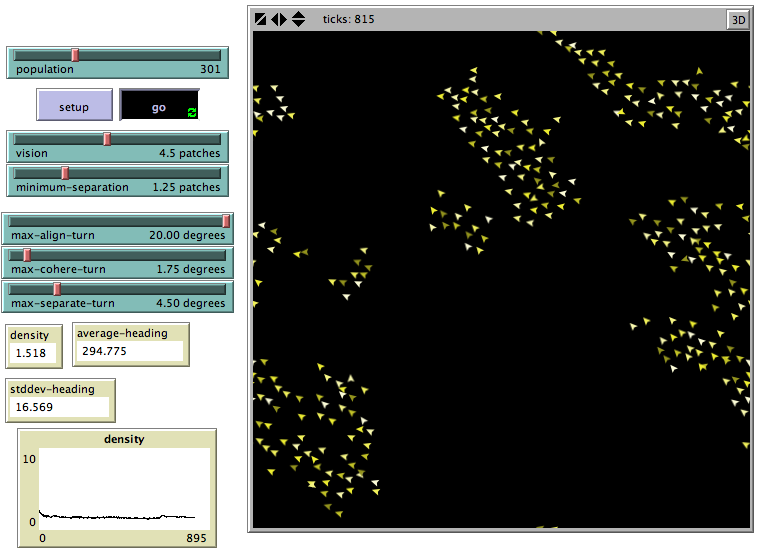
\includegraphics[scale=.333333]{images/flocking_ss.png}
\caption{Screen capture of the NetLogo Flocking ABM.}
\label{fig:flockingss}
\end{figure}

The NetLogo implementation of flocking follows the original definition closely.
There are six configuration parameters, as seen in Figure \ref{fig:flockingss}, however, only three are used:
\begin{itemize}
\item \textit{max-align-turn} -- the maximum amount of degrees an agent will turn to align heading with its neighbors,
\item \textit{max-cohere-turn} -- the maximum amount of degrees an agent will turn towards the center of the flock,
\item \textit{max-separate-turn} -- the maximum amount of degrees an agent will turn away if another agent is within \textit{minimum-separation}.
\end{itemize}
The other three configuration parameters available in the user interface (\textit{population}, \textit{vision}, and \textit{minimum-separation} are excluded because they do not affect the system-level properties as directly as the three outlined above.
The values for these parameters are kept constant throughout the experimentation performed for this thesis.

Two system-level properties are analyzed for this system:
\begin{itemize}
\item \textit{spread} -- measures how spread out the agents are.

This metric is calculated as the average distance from each agent to its nearest neighbor.
This calculation is an approximation to the true density, as it does not directly measure agents per patch.
Approximating is necessary because determining the area that an individual flock covers is not trivial and sometimes subjective.
In addition, a single instance could have several individual flocks, making this computation even more obscure.
The distance to the average neighbor captures the information that density conveys: as the distance increases, the agents are more spread out, and thus less dense.

\begin{figure}[ht]
\centering
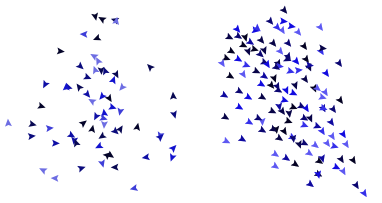
\includegraphics[scale=1]{images/swarmVSflock.png}
\caption{A swarming boid system (left) and a flocking boid system (right).}
\label{fig:swarmVSflock}
\end{figure}

\item \textit{stddev-heading} -- measures the standard deviation of the agent headings.

This metric is used to determine how much the agents in the ABM agree on the direction they are heading.
Configurations with agents that flock smoothly in one direction typically have a very low \textit{stddev-heading} value.
Meanwhile, more chaotic configurations will have a relatively high \textit{stddev-heading} value.
This contrast is illustrated in Figure \ref{fig:swarmVSflock}.

\end{itemize}

The Flocking ABM has the role that it is less challenging than Wolf Sheep Predation, but more complex than Fires.
The system-level properties change in a more monotonic and predictable manner than the other domains, but still remains sufficiently complex.
The behaviors are not linear and the configuration space is three-dimensional, making this problem still nontrivial. 

%%%%%%%%%%%%%%%%%%%%%%%%%%%%%

\section{NetLogo AIDS}

The AIDS ABM is a model of how AIDS spreads in humans.
There are a number of agents in a two-dimensional world that move around randomly.
Agents that collide have a chance to couple, and have a chance to spread AIDS if one partner has AIDS (\textit{HIV+} and one does not (\textit{HIV-}).
Individuals that know they have the disease will not spread it to people without it.
Only individuals that have AIDS but do not know (\textit{HIV?}) can spread the disease.
Eventually, once there are no more people unknowingly spreading AIDS, the population is segregated into people who have AIDS and know it, and people that do not have it.
A screen capture of the domain running in NetLogo is shown in Figure \ref{fig:aidsss}.

\begin{figure}[ht]
\centering
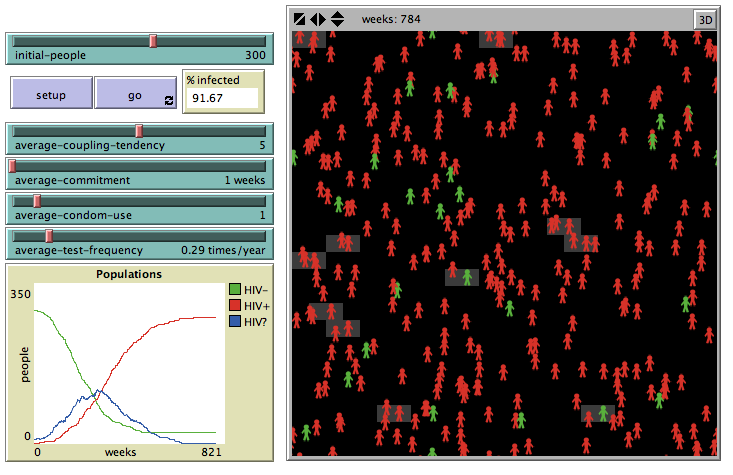
\includegraphics[scale=.5]{images/aids_ss.png}
\caption{Screen capture of the NetLogo AIDS ABM.}
\label{fig:aidsss}
\end{figure}

\begin{figure}[ht]
\centering
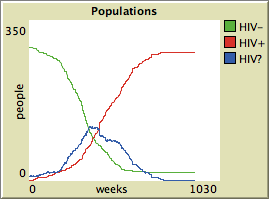
\includegraphics[scale=.666667]{images/condom_low.png}
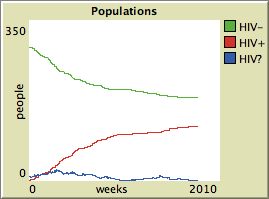
\includegraphics[scale=.666667]{images/condom_high.png}
\caption{Plot of a AIDS ABM run with low (left) and high (right) \textit{average-condom-use} (notice the difference in the scale of weeks).}
\label{fig:aids_condom}
\end{figure}

\begin{figure}[ht]
\centering
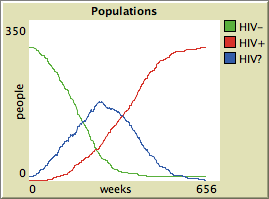
\includegraphics[scale=.666667]{images/test_low.png}
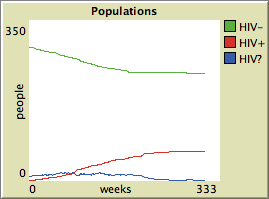
\includegraphics[scale=.666667]{images/test_high.png}
\caption{Plot of a AIDS ABM run with low (left) and high (right) \textit{average-test-frequency} (notice the difference in the scale of weeks).}
\label{fig:aids_test}
\end{figure}


There are five configuration parameters available in the NetLogo implementation of this ABM.
However only two are used for the intents of this dissertation:
\begin{itemize}
  \item \textit{average-condom-use} -- The probability that one of the two individuals will insist on using a condom.

The usage of a condom prevents the spread of the disease.
Therefore, when this value is lower, the disease will spread to more people.
When this value is higher, the opposite happens.
The difference between a high value and a low value is illustrated in Figure \ref{fig:aids_condom}.

  \item \textit{average-test-frequency} -- The frequency that an individual will get tested for AIDS, per year.

Getting tested decreases the population of the individuals that have AIDS but do not know it, directly reducing the number of agents capable of spreading the disease.
This parameter has as similar effect as \textit{average-condom-use}, as seen in Figure \ref{fig:aids_test}.
\end{itemize}
The other parameters, \textit{initial-people}, \textit{average-coupling-tendency} (chance a couple will form), and \textit{average-commitment} (how long a couple stays together) are not used.
I chose not to incorporate these in my experiments because they change the system-level behavior in a similar way to the two parameters that I do use.
In addition, condom usage and test frequency may be more easily affected by public policy than coupling tendency and how long a couple are committed for.

For this domain, I will use \fw to model the plots of the populations, such as the ones in Figures \ref{fig:aids_condom} and \ref{fig:aids_test}.
This is done by using a parametric model to perform curve fitting (i.e., nonlinear regression) on training instances and extracting the model parameters as the system-level properties.
Thus, the forward mapping maps the two configuration parameters to predicted values of the parameters of the model.
A prediction of what the plots will look like can then be predicted with the forward mapping.
A base parametric model is needed that can fit the data well.

For this domain, the curves appear to be sigmoid functions, so I will use a generalized logistic function:
\[P(t) = c_1 + \displaystyle\frac{c_2 - c_1}{1 + e^{-c_3 (t - c_4)}}.\]
The parameters indicate the following:
\begin{itemize}
 \item $c_1$ -- the lesser asymptote,
 \item $c_2$ -- the greater asymptote,
 \item $c_3$ -- the growth rate, and
 \item $c_4$ -- the location of the inflection point.
\end{itemize}

The step of performing the nonlinear regression to model the curve is done after the raw data sampling and before solving the forward mapping.
Each instance of scatter plot data has nonlinear regression applied to it to determine the four parameters of the logistic function.
The parameters are used as the new data set, instead of the original scatter plot data.

In conclusion, the AIDS domain is used to specifically demonstrate the usage of parametric models to describe system-level behaviors over time.



%%%%%%%%%%%%%%%%%%%%%%%
 \section{NetLogo Wolf Sheep Predation}
The NetLogo Wolf Sheep Predation ABM has been the running example throughout this dissertation.
In this ABM, there are three major entities: wolves, sheep and grass.
Wolves eat sheep, sheep eat wolves and sheep eat grass.
The grass naturally regrows, meanwhile wolves and sheep occasionally reproduce.
Every time step sheep and wolves lose some energy and die naturally if their energy reaches zero.
A screen capture of the Wolf Sheep Predation ABM in NetLogo is shown in Figure \ref{fig:wolfsheepss}.
The configuration controls are in the top left, the monitors are in the bottom left and the visualization of the domain is on the right.

\begin{figure}[ht]
\centering
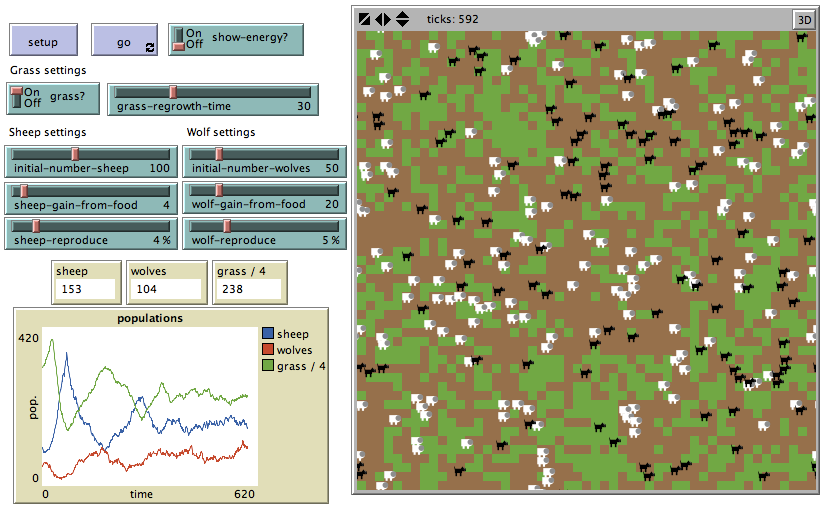
\includegraphics[scale=.4]{images/wolfsheep_ss.png}
\caption{Screen capture of the Wolf Sheep Predation ABM.}
\label{fig:wolfsheepss}
\end{figure}

The populations of a running Wolf Sheep Predation system are constantly changing.
Therefore, measuring properties is not as straightforward as in the Fires ABM.
Changes in populations can range from small oscillations to high magnitude oscillations in numbers, depending on the configuration parameters.
Quantitatively capturing these properties is challenging, but is possible with \fw.
A plot of a relatively normal (not too stable and not too high-magnitude) population is shown in Figure \ref{fig:wsp_norm}.

\begin{figure}[ht]
\centering
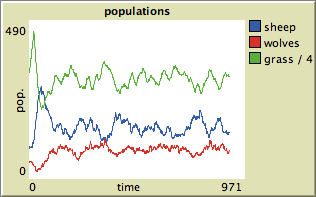
\includegraphics[scale=.666667]{images/wolfsheep/wolfsheep_normal.png}
\caption{Plot of a stable populations in a Wolf Sheep Predation system.}
\label{fig:wsp_norm}
\end{figure}


\begin{figure}[ht]
\centering
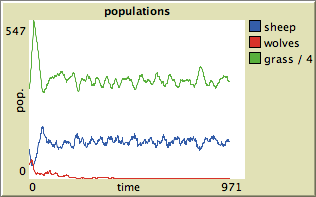
\includegraphics[scale=.666667]{images/wolfsheep/sheepfood_low.png}
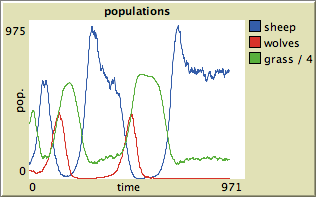
\includegraphics[scale=.666667]{images/wolfsheep/sheepfood_high.png}
\caption{Plot of a Wolf Sheep Predation run with low (left) and high (right) \textit{sheep-gain-form-food}.}
\label{fig:wsp_sheepfood}
\end{figure}


\begin{figure}[ht]
\centering
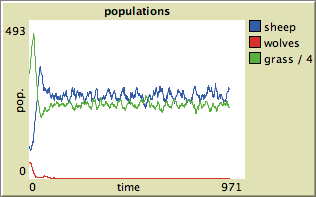
\includegraphics[scale=.666667]{images/wolfsheep/wolffood_low.png}
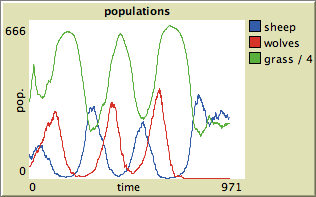
\includegraphics[scale=.666667]{images/wolfsheep/wolffood_high.png}
\caption{Plot of a Wolf Sheep Predation run with low (left) and high (right) \textit{wolf-gain-form-food}.}
\label{fig:wsp_wolffood}
\end{figure}


\begin{figure}[ht]
\centering
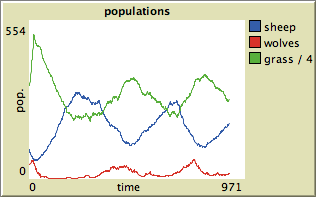
\includegraphics[scale=.666667]{images/wolfsheep/sheepsex_low.png}
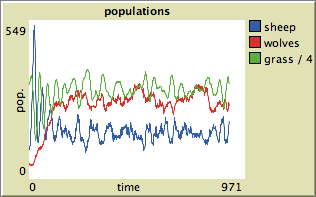
\includegraphics[scale=.666667]{images/wolfsheep/sheepsex_high.png}
\caption{Plot of a Wolf Sheep Predation run with low (left) and high (right) \textit{sheep-reproduce}.}
\label{fig:wsp_sheepsex}
\end{figure}


\begin{figure}[ht]
\centering
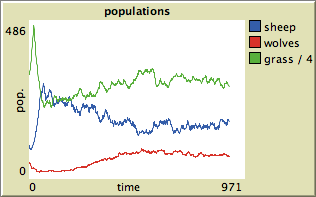
\includegraphics[scale=.666667]{images/wolfsheep/wolfsex_low.png}
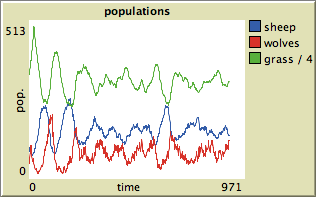
\includegraphics[scale=.666667]{images/wolfsheep/wolfsex_high.png}
\caption{Plot of a Wolf Sheep Predation run with low (left) and high (right) \textit{wolf-reproduce}.}
\label{fig:wsp_wolfsex}
\end{figure}


The configuration space is five-dimensional, making this domain nontrivial to analyze.
The configuration parameters, along with some general observations, are as follows:
\begin{itemize}
   \item \textit{sheep-gain-from-food} -- the amount of energy sheep gain from eating grass.
This parameter has interesting effects on the system.
The effect of changing this parameter from the stable norm is shown in Figure \ref{fig:wsp_sheepfood}.

At lower values, the population of the sheep has difficulty not going extinct.
This almost always results in the wolf population going extinct.

At higher values, sheep live longer and quickly become overpopulated, which causes the grass to become a scarce resource.
With little grass left, the sheep begin to die off.
Once enough sheep have died off, the grass begins to regrow and the sheep begin to reproduce.
This results in sharp increases and decreases in sheep population as the sheep population oscillates between overpopulated and underpopulated.
When the oscillations are of high enough magnitude, the wolves have a high chance of becoming extinct while the sheep population is very low.


   \item \textit{wolf-gain-from-food} -- the amount of energy wolves gain from eating a sheep.
This parameter affects the system in a similar way as \textit{sheep-gain-from-food}.
Lower values cause the wolves to go extinct, while higher values cause more drastic oscillations in wolf and sheep populations.
The effect of changing this parameter from the stable norm is  shown in Figure \ref{fig:wsp_wolffood}.

   \item \textit{sheep-reproduce} -- the percent chance that a sheep will reproduce, per time step.
This parameter has the interesting property that when it is increased, the wolf population increases, but the sheep population remains relatively constant.
When \textit{sheep-reproduce} is too low, the sheep population has difficulties sustaining its numbers, which causes the wolf population to be very low.
The effect of changing this parameter from the stable norm is  shown in Figure \ref{fig:wsp_sheepsex}.

   \item \textit{wolf-reproduce} -- the percent chance that a wolf will reproduce, per time step.
This parameter has relatively little effect on the system, in comparison to the other parameters.
The populations oscillate more when the reproduction rate is higher and more stable with it lower.
The effect of changing this parameter from the stable norm is  shown in Figure \ref{fig:wsp_wolfsex}.

   \item \textit{grass-regrowth-time} -- the amount of time steps a patch of grass takes to regrow.
This is perhaps the strangest behaving configuration parameter.
At higher values, not enough grass grows to sustain a large sheep population, which causes the wolves to go extinct.
At lower values, sheep rarely every die, until they become overpopulated and eat all the grass.
At this point, there is a mass extinction, which causes the wolves to typically go extinct.
In behavior, this parameter is similar to that of \textit{sheep-gain-from-food}.

\end{itemize}
Each of these parameters individually affect the system state.
Even more diverse behaviors can be observed by adjusting several parameters at once.

Several system-level properties have been developed for this domain.
To sample many of these properties and to provide more consistent results, each random configuration is sampled a number of times and averaged.
\begin{itemize}
\item \textit{sheep-extinct?} and \textit{wolves-extinct?} -- the probability that the sheep and wolf populations will reach zero, respectively.

The probability of sheep and wolf extinction is measured by sampling the same configuration numerous times and calculating the percentage of instances they went extinct.
Most often with a specific configuration, the sheep or wolves always go extinct or always do not go extinct.
However, there are borderline configurations in which the sheep or wolves will go extinct while the system is stabilizing into a rhythm.
This metric is useful in distinguishing between these three situations.
Wolves will always go extinct if there are no sheep, but sheep can exist without wolves.
Therefore, the value of \textit{wolves-extinct} is always higher than \textit{sheep-extinct?}.

\item \textit{sheep-average} and \textit{wolf-average} -- the average sheep and wolves given they did not go extinct, respectively.

The average sheep and wolf populations are calculated by averaging the populations at every time step in instances in which they did not go extinct.
Not including extinct populations in the average is important because these instances will introduce significant amounts of bias.
This metric describes how large the population can expected to be.
Along with \textit{sheep-variance} and \textit{wolf-variance}, the averages describes the nature of the population and how it changes.

\item \textit{sheep-variance} and \textit{wolf-variance} -- the variance of the sheep and wolf population over the course of a run.

The variance is calculated with the same data as the average.
This metric describes how much the population changes from time step to time step, since the population is typically rhythmically changing.

\end{itemize}

The Wolf Sheep Predation ABM is interesting because its behaviors are not linear and are not monotonic.
That is, as many of the configuration parameters increase, the resulting system-level behavior does not change in a linear manner.
This property of the behavior space makes many of the system-level properties difficult to predict.
In addition, there are five configuration parameters, which makes the configuration space five-dimensional.
The system-level property space is up to six dimensions.
Handling dimensionality up to eleven is a challenging task for any approach that is attempting to analyze system-level behavior.




\cleardoublepage

\chapter{THE FORWARD MAPPING PROBLEM}
\thispagestyle{plain}

\label{ForwardMapping}

% the forward mapping problem asks to develop a mapping from configuration space to system-level property space
% This chapter details aspects of the forward mapping problem and the proposed solution used in \fw.
% Also, evaluation criteria for solutions to the FMP is given.

\section{Definition of the Problem}
% develop an accurate mapping from //configuration space// to //system-level property space//.
% This entire mapping describes what is called the //behavior space//.

% configuration space consists of any number of ABM parameters that change the behavior
% Configuration parameter values can be discrete values (i.e., integers) or real values
% Thus, this space is n-dimensional, each dimension representing a single configuration parameter

% The system-level property space consists of all properties wanting to be measured.
% this space has one dimension per property to be measured.
% Typically, these values are always real valued. 
% Since it is a prediction, an impossible value (i.e., expected discrete value) still has meaning... for example the number of wolves expected could be 69.7, which is obviously impossible to have .7 wolves, but still shows that the value tends to be closer to 70 than 69, more often than not.

% A solution must be able to handle highly dimensional spaces and must be able to handle continuous and discontinuous configuration spaces.
% Also, several evaluation criteria that could be used to analyze the effectiveness and efficiency of solutions are provided later in this chapter.


\section{The \fw Approach}

% The default approach taken by \fw to solve the forward-mapping problem is to do regression
% Regression fits this problem naturally, as regression takes indp variables and generates possible values for dep variables.
% The configuration parameters are the independent variables and the system-level properties are the dependent variables.

% The sampling phase provides a data set with several instances of configuration, outcome observation pairs.
% These are provided to the regression algorithm to base its predictions off of.
% Different regression approaches use this data in different ways.
% Approaches like KNN do no pre-processing at all and uses the entire data set for each query.
% Meanwhile, approaches like Nonlinear Regression train a compact parametric model to represent the data and does not require the data set after this point.
% In general, more time spent pre-processing equates into less time querying, but is not proportionate. 

% Other possible approaches fall into the field of machine learning.
% Approaches such as kernel methods and neural networks could solve the similar prediction problem here, but regression was selected particularly to make solving the reverse mapping problem, which is discussed in the next chapter.

\subsection{Scaling}
% Scaling the data set is an important factor in learning the forward mapping.
% The problem is that the different configurations have different ranges and different meanings.
% Performing a simple euclidean distances on these is not sufficient, since the closeness of points will often be skewed on the values.
% For example, consider a percentage value in the WS domain (sheep birth rate, which may be sampled 1-8% or .01 to .08) and sheep-gain-from-food from 2-10.
% The euclidean metric treats all dimensions as equal, so closeness in the larger ranged dimension will give higher weight than closeness in the smaller ranged dimension

% Typically, simply scaling each dimension such that the minimum value experienced is zero and the highest value is one, and then scaling all others accordingly works fine.
% However, more advanced techniques such as X, Y, Z have their advantages.
% A more in depth analysis on the effects of these approaches to the effectiveness of different approaches is left as future work (See \ref{sec:fw_scaling})

% The choice of scaling technique and distance metric is determined in the scope of the regression algorithm used, particularly in the training step.
% For example, KNN could preprocess the dataset into a scaled data set for future use.


\subsection{Handling Non-Continuous Configuration Spaces}
% In the original problem statement, I mentioned that the configuration space could contain discrete values.
% These discrete valued configuration parameters typically represent numbers of agents.
% The reason for the real-value assumption is just to simplify the process.

% The limitations introduced by this assumption can easily be circumvented in a number of different ways.
% First, the value can simply be rounded to the nearest integer value to produce integer values.
% The challenge in this approach is not sampling, but how the regression approaches will handle non-continuous spaces, in the case that they are expecting continuous spaces.
% For example KNN and to a lesser extent other nonparametric methods such as LOESS are agnostic to this problem.

% In continuous domains, the distance metric must be chosen with care
% since random configurations will be chunked into discrete groups.
% points within the same discrete value group may naturally weight one another higher since they are equal in one dimension.
% This could be bad for a technique such as k-nearest neighbor.
% In KNN, the nearest neighbors may always be colinear values and completely ignore the non-discrete dimensions.
% This problem is illustrated in Figure X.
% [[ MAKE A FIGURE: show a 2d map of the distributions of a random sample. show that ''rows'' form. Show what the kNN would be for a particular point, and show that all of those points are in the same row.
% The simplest way to solve this problem is to scale the discrete distances such that they are similar to the average distance between colinear points in a discrete parameter.
% If the samples were taken randomly and the space is scaled to a square, which is the default behavior for \fw, this property is natural.

\subsection{Handling Multi-Variate Forward Mappings}

% In the definition of the problem, I mention the fact that a number of system-level properties can be measured at once.
% To handle this, I split each system-level property into its individual single-property forward mapping problem.
% give some math that splits the vector y into several individual ys

% The alternative to this would be to use a multi-variate regression approach, such as X.
% The main difference between these multi-variate approaches and my approach, is I have to assume that the dependent variables are statistically independent, i.e., they don't affect each other.
% This assumption may not always be the case, but I have not personally found this to be a problem in any of the ABMs I have experimented with.
% Also, the ability to use simple single-variate regression algorithms broadens the flexibility of the approach, makes it easier to implement and simplifies the solution to the reverse-mapping problem.
% An investigation for the effectiveness of multi-variate regression approaches for this research is left as outside the scope of this dissertation.

\subsection{Implementation Details}

% The solution to the forward mapping problem in \fw is split into two distinct steps: training and predicting.
% training builds the model and/or preprocesses the data as necessary.
% The predicting program allows the user or other components of the framework to query the regression model
% This process is assisted by a user-provided regression library that is used to build the models.
% More on how to build the module property to interface with \fw, see Appendix ??.

\subsubsection{Training}

% The training portion of solving the forward mapping is where any necessary necessary preprocessing and/or model building is done
% Also, scaling of the data can be done in this step.
% This is implemented as a Python program called train.py. train.py takes in the data set generated by the sampling as well as a user-created regression module that was built to interface with train.py.
% train.py then passes the data set to the regression module, which then may produce model files on the local filesystem.

% KNN may simply just scale the data, or with more advanced implementations build a geo hash or kd-tree.
% LOESS will perform the locally weighted smoothing step to build $y'$ values. (and output the smoothed data set)
% NLR will learn optimal parameters for the parametric model given with optimization. (and output the parameters)
% MLI will build a evenl spread data set with another regression algorithm
% Each of these approaches require varying computational time



\subsubsection{Predicting}

% The prediction step is the step in which queries are passed and predictions are returned.
% This is implemented as a python program predict.py that takes the regression module and any trained meta-data to generate predictions (answers to user-specified queries)
% Any number of queries in the form of a configuration vector are passed in through standard in, with answered returned in standard out.

% KNN will iterate through every point to find the kNN, then average the values
% LOESS will interpolate between nearby smoothed data set points to determine the new value
% NLR will simply plug in values for the configuration parameters and calculate the result
% MLI will find which bin the point lies within and then interpolate from the corners.


\section{Using the Forward Mapping Models}

% The forward mapping model has two main uses: prediction of behavior for a user and used by \fw for the reverse mapping.
% A user can use the forward mapping to predict the behavior of a system without having to run it.
% This could be useful for a number of reasons: it may be faster, it may be more convenient.
% Thus, this approach is more useful than interacting with the ABM directly to varify hypotheses about behavior, answering 'what-if' questions and manually exploring the behavior space faster.

% \fw uses the forward mapping to solve the reverse mapping.
% A number of approaches are discussed in Chapter \ref{ReverseMapping}: The Reverse-Mapping Problem, but practically all use the forward mapping instead of direct sampling for the same reasons the user uses this over it.
% The forward mapping describes behavior faster than direct sampling, and allows faster searching of the space to answer queries.

% A secondary use for the forward mapping would be to plot the behavior space or visualize the behavior space in different ways.
% Plotting programs do not calculate the value for every point (there are infinite!), what they typically do is sample a bunch of points then interpolate between them.
% the forward mapping can be used for this purpose: to generate a bunch of points, then plot lines between them.
% Also, parametric regression approaches (NLR) could be graphed directly and even compared to the training (or validation) set.



\section{Solution Evaluation Criteria}

% An important step in generating a solution for the forward mapping problem is evaluating it.
% I propose a single core approach, which I will be evaluating, with these criteria, in Chapter \ref{Results}.

% Each of the following criteria have different weight, but are all important in their own way.

\subsection{Time Required for Training}

% The time required for training is listed as not very important in my original design goals.
% However, intractable training problems should be avoided.

% There are two matters of importance when measuring the time required for training a model.
% First, how long does it take
% Second, how does the length of time scale with larger data sets (quadratic? exponential? linear?)

% Measuring how long it takes is easy: just measure the amount of time
% The second is easy as well, just measure in comparison to the data set size.


\subsection{Time Required for Querying}

% Time required for querying is noted as important in the design goals.
% In fact, time required for querying should ALWAYS be below the amount of time it takes to just sample the ABM.
% If it is longer, there is no point and the user would just sample the ABM directly, instead of use \fw.

% To measure this, a large number of random queries are passed to the regression algorithm, and statistics such as average response time and standard deviation of response times can be used to evaluate the speed of these approaches.
% The speed of querying the system is used as a baseline to compare to in experiments.

% In some cases/algorithms, the size of the data set may effect the time required for querying.
% This relationship should also be evaluated to determine at which point direct domain sampling would be better.


\subsection{Accuracy of the Forward Mapping}
% The accuracy of the forward mapping is perhaps the most important of all evaluation criteria.
% If the mapping is not accurate, it is not useful.
% There is a certain amount of error that is tolerable for the increased speed of predicting values in \fw, 
% however, the error cannot be too high.

% To measure the accuracy of the predictions, two approaches are possible.
% First, cross validation can be used to split the training set into a training set and a validation set.
% Another, but slower approach, is the predict the value for a configuration and then actually run the simulation, and compare the values.

% The errors calculated for an entire run are summed for a total accumulated error.
% The higher the sum, the worse the predictor.
% Other properties including the standard deviation of errors could be useful as well.
% Visualizing the distribution of errors could also be useful in detecting a bias in prediction.
% Visualizing the error localized to specific parts of the configuration space could show which areas of the space are less predictable or could require more sampling.


\subsection{Data Set Size Requirement}

% The size of the data set required to make accurate predictions is an important factor.
% The data set takes a significant amount of time to sample, so smaller data set requirements are better.

% Also, knowing what size data set is appropriate for a given domain and given algorithm is important for designing new experiments for use in \fw.

% This is measured by calculating the ``Accuracy of the Forward Mapping" errors, but comparing the change of this error to the size of the data set.
% Typically, error should decrease as the sample size increases.




\cleardoublepage

\chapter{THE REVERSE MAPPING PROBLEM}
\thispagestyle{plain}

\label{ReverseMapping}

Lorem ipsum dolor sit amet, consectetur adipisicing elit, sed do eiusmod tempor incididunt ut labore et dolore magna aliqua. Ut enim ad minim veniam, quis nostrud exercitation ullamco laboris nisi ut aliquip ex ea commodo consequat. Duis aute irure dolor in reprehenderit in voluptate velit esse cillum dolore eu fugiat nulla pariatur. Excepteur sint occaecat cupidatat non proident, sunt in culpa qui officia deserunt mollit anim id est laborum.



\cleardoublepage

\chapter{RESULTS}
\thispagestyle{plain}

\label{Results}

In this chapter, I discuss experiments that test \fw for accuracy and computational efficiency.
These experiments also serve as examples of \fw being applied to a variety of ABMs.
In the next section, the different evaluation criteria are outlined.
Each of these metrics will be applied to a number of domains using a number of different techniques for the forward mapping.
The four domains used for the sake of experimentation are outlined in Section \ref{sec:tdomains}: Target Domains.
Each of these domains have unique properties that provide unique challenges to show the versatility of \fw.
The different regression methods for the forward mapping are outlined in Section \ref{sec:fmalgo}: Forward Mapping Methods.
Finally, in Section \ref{sec:exps}: Experiments, the statistical results are discussed.

\section{Evaluation}

Evaluating \fw is important to show that \fw is a practical and useful tool for studying ABMs.
Evaluation is split into two processes: evaluating the forward mapping solution and evaluating the reverse mapping solution.
Accuracy of these mappings in modeling the behavior space of the target ABM is paramount in importance.
If the meta-models are not accurate, there would be no reason to use this framework for investigating behaviors of ABMs.
Computation time is also an important factor in evaluating \fw.
Interactions with the user need to be quick in order to make using \fw more convenient than manually inspecting the target ABM.
The response time of when a user interacts with \fw is the \textit{online} time and is far more important than the \textit{offline} time, the one-time computation requirement to learn the forward or reverse mapping.


 \subsection{Forward Mapping}

  \subsubsection{Accuracy}
Accuracy is the measurement of how closely the forward mapping represents the true behavior space of a target ABM.
To measure this, the difference (error) $\varepsilon$ between the predictions for a system level property $\hat y$ that the forward mapping produces and the actual value $y$ for a sampled point: $\varepsilon = |\hat y - y|$.
This measurement is performed many times for a single domain to produce the average error $\bar \varepsilon$ and the the standard deviation of the errors $\sigma$.

Measuring the error is done by performing cross validation.
Two subsets of data points are randomly pulled from the master set of samples to create a training set and a validation set.
The forward mapping is built by using the training set, and then checked with the validation set.

The error is calculated for varying size data sets to show the relationships between error and data set size.

  \subsubsection{Offline Computation Time}

Offline computation time is the average amount of system time the forward mapping uses to train a model.
This is measured as the amount of time the pre-processing takes, given a training set.
The size of the training set is varied to determine how forward mapping training time is correlated to training set size.
Each forward mapping methods is compared to the others.

  \subsubsection{Online Computation Time}

Online computation time is the average amount of time \fw takes to return the results of a user-submitted query.
This is measured by performing a large number of random queries and calculating the average run time.
The size of the training set can affect the amount of time a query will take with some algorithms.
In these cases, the size of the training set is varied to determine how query time correlates to training set size.

 \subsection{Reverse Mapping}

  \subsubsection{Accuracy vs. Forward Mapping}
Accuracy of the reverse mapping is measured in two ways.
The first is how accurately the reverse mapping models the forward mapping.
Recall that \fw solves the reverse mapping by building an invertible approximation of the forward mapping.
This metric determines if this approach is doing what is expected to do.
The effect that granularity has on this accuracy is also measured by learning the same mapping with increasingly higher granularity.

\begin{figure}[ht]
\centering
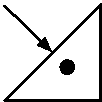
\includegraphics[scale=1]{images/mosterror.pdf}
\caption{The most erroneous spot in a right-angled simplex.}
\label{fig:mosterror}
\end{figure}

The error is presented as an ``average worst-case scenario".
The area of the reverse mapping space that is be the most erroneous is typically be the one furthest from the knots (corners of the simplex).
An illustration of this point is presented in Figure \ref{fig:mosterror}.
The point is halfway between all corners, except for the corner at the right angle.
This point is the most erroneous if the forward mapping is monotonically changing from one side of the simplex to the other (i.e., there are no local maxima or minima within the space).
Note that the reverse mapping will be identical to the forward mapping at the knots, since the forward mapping was used to infer their values.

Calculating the approximate upper bound on error, within a simplex, involves interpolating the system-level property value at the most erroneous point.
This is done by average the system-level property values of all corners not at the right angle.
Also, the location of the most erroneous point is queried for prediction through the forward mapping.
The difference between the interpolated value on the simplex and the actual predicted value using the forward mapping constitutes the error.
This metric is applied for every simplex and then averaged.
Thus, the metric measures the average error over all the worst-case scenarios for each simplex.
Also, the standard deviation of these errors is provided to convey how consistent the reverse mapping is.


  \subsubsection{Accuracy vs. Agent-Based Model Run}

The main goal of the reverse mapping is to be able to suggest configurations that would generate this behavior.
This approach is different from the previous metric because it measures the difference between the reverse mapping and the true behavior space.

\begin{figure}[ht]
\centering
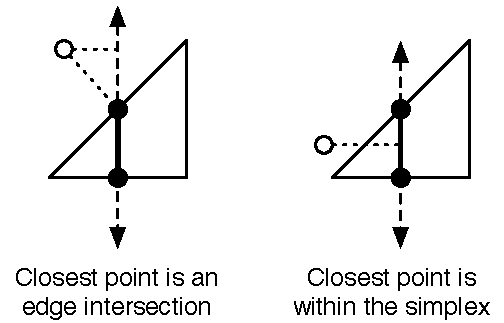
\includegraphics[scale=1]{images/closest.pdf}
\caption{Two cases for the closest point to a simplex intersection.}
\label{fig:closest}
\end{figure}

Error is measured by generating a random configuration point and sampling it from the agent-based model.
Then, the system-level property that was measured is passed to \fw to generate a reverse-mapping solution.
The error is the distance from the original configuration and the reverse-mapping solution space.
This value is calculated by adhering to the following procedure, per simplex:
\begin{enumerate}
  \item Determine the distance from the original point to the intersecting hyperplane.
  \item If the shortest line from the hyperplane to the point intersects the hyperplane \textit{within} the simplex, then the distance from the hyperplane is the distance from the intersection to the point.
  \item Otherwise, the closest point is one of the edge intersections.
\end{enumerate}
The two different cases (closest to an edge (left) and closest to the hyperplane (right)) are illustrated in Figure \ref{fig:closest}.
Then, the minimum from all these closest points is taken as the distance from the actual system-level property value and the value provided by the reverse mapping.
This distance is the error.

Several random configurations are sampled in this way.
The average and standard deviation of these errors are calculated to convey the accuracy of the reverse mapping, as well as the consistency of the reverse mapping.

  \subsubsection{Offline and Online Computation Time}
Offline computation time and online computation time is measured the same way for the reverse mapping as the forward mapping.
The amount of time \fw takes to prepare the reverse mapping is the offline computation time, and the amount of time required to produce a reverse mapping solution is the online computation time.





\section{Target Domains}\label{sec:tdomains}

Four target domains are used to show \fw effectiveness in a variety of different types of situations.
No modifications to \fw have to be performed to have \fw compatible with these domains.
This shows that \fw is domain independent.

 \subsection{NetLogo Fires}\label{sec:Fires}



\begin{figure}[ht]
\centering
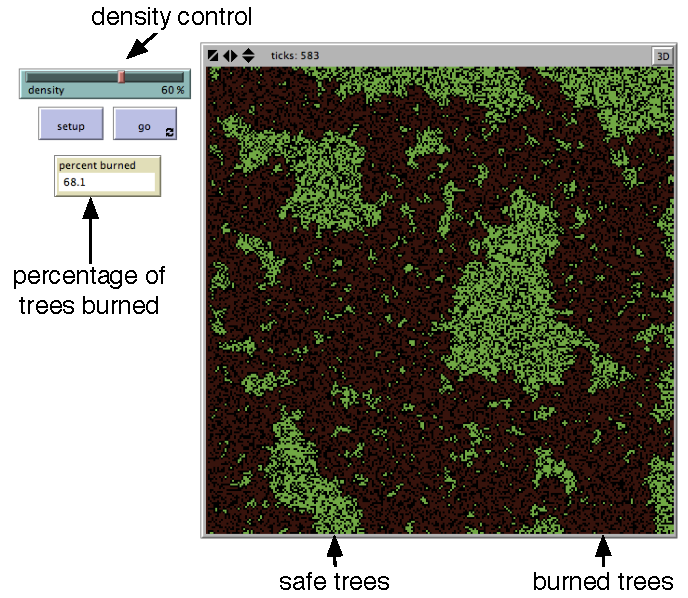
\includegraphics[scale=1]{images/fires_ui.pdf}
\caption{Screen capture of the Fires NetLogo ABM.}
\label{fig:firesui}
\end{figure}

The NetLogo Fires ABM is the simplest ABM tested in this dissertation.
In this ABM, trees are distributed throughout a $250 \times 250$ grid world.
A fire is started in the left column, in which all trees in this column burn.
Each burning tree then burns its adjacent trees (up, down, left, and right).
This process continues until no more trees are adjacent to burning trees.

The configuration space is one-dimensional and the system-level property space is one dimensional.
The configuration parameter for this domain is the density $\rho$ of the forest, which in our experiments I range from 45 \% to 75\%.
What this parameter does is change the probability that a grid point contains a tree.
During the initialization step, each grid point has a tree placed with probability $\rho$.
The system-level property is the percentage of trees burned down, which is measured by diving the number of trees that were burned by the total number of trees in the system.


The Fires ABM is particularly interesting because it exhibits a threshold effect.
There is a sharp transition from small amounts of the forest burning down and the entire forest burning down when the forest density increases past 58\%.
The behavior space is not linear and exhibits high variance around 58\%, making this ABM moderately challenging, regardless of it only having one configuration parameter.

The Fires ABM is used as an example in this chapter on how to apply every aspect of \fw to a single domain later on in this chapter.


 \subsection{NetLogo Wolf Sheep Predation}
The NetLogo Wolf Sheep Predation ABM has been the running example throughout this dissertation.
In this ABM, there are three major entities: wolves, sheep and grass.
Wolves eat sheep, sheep eat wolves and sheep eat grass.
The grass naturally regrows, meanwhile wolves and sheep occasionally reproduce.
Every time step sheep and wolves lose some energy and die naturally if their energy reaches zero.
A screen capture of the Wolf Sheep Predation ABM in NetLogo is shown in Figure \ref{fig:wolfsheepss}.
The configuration controls are in the top left, the monitors are in the bottom left and the visualization of the domain is on the right.

\begin{figure}[ht]
\centering
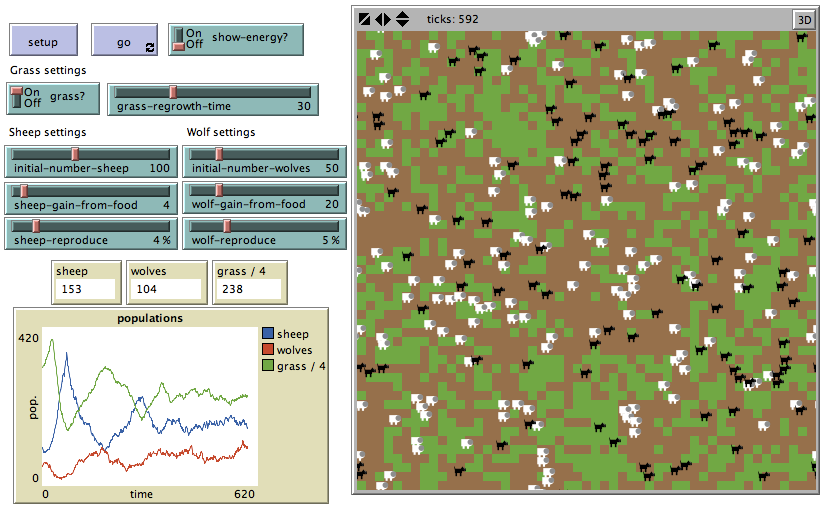
\includegraphics[scale=.4]{images/wolfsheep_ss.png}
\caption{Screen capture of the Wolf Sheep Predation ABM.}
\label{fig:wolfsheepss}
\end{figure}

The populations of a running Wolf Sheep Predation system are constantly changing.
Therefore, measuring properties is not as straightforward as in the Fires ABM.
Changes in populations can range from small oscillations to high magnitude oscillations in numbers, depending on the configuration parameters.
Quantitatively capturing these properties is challenging, but is possible with \fw.
A plot of a relatively normal (not too stable and not too high-magnitude) population is shown in Figure \ref{fig:wsp_norm}.

\begin{figure}[ht]
\centering
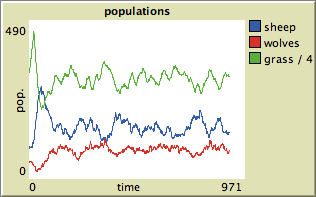
\includegraphics[scale=.666667]{images/wolfsheep/wolfsheep_normal.png}
\caption{Plot of a stable populations in a Wolf Sheep Predation system.}
\label{fig:wsp_norm}
\end{figure}


\begin{figure}[ht]
\centering
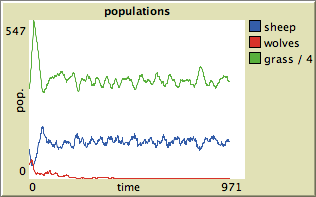
\includegraphics[scale=.666667]{images/wolfsheep/sheepfood_low.png}
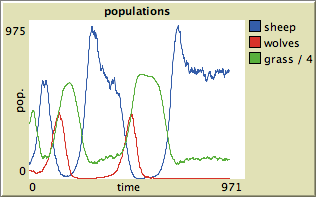
\includegraphics[scale=.666667]{images/wolfsheep/sheepfood_high.png}
\caption{Plot of a Wolf Sheep Predation run with low (left) and high (right) \textit{sheep-gain-form-food}.}
\label{fig:wsp_sheepfood}
\end{figure}


\begin{figure}[ht]
\centering
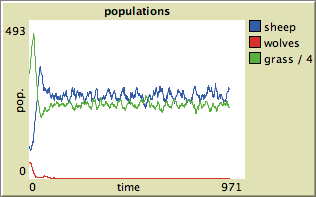
\includegraphics[scale=.666667]{images/wolfsheep/wolffood_low.png}
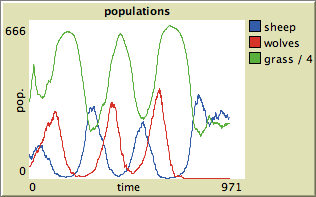
\includegraphics[scale=.666667]{images/wolfsheep/wolffood_high.png}
\caption{Plot of a Wolf Sheep Predation run with low (left) and high (right) \textit{wolf-gain-form-food}.}
\label{fig:wsp_wolffood}
\end{figure}


\begin{figure}[ht]
\centering
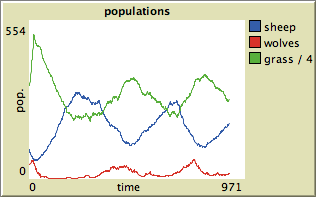
\includegraphics[scale=.666667]{images/wolfsheep/sheepsex_low.png}
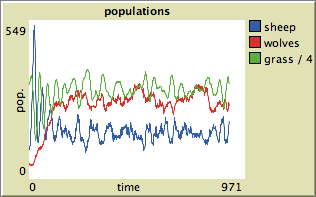
\includegraphics[scale=.666667]{images/wolfsheep/sheepsex_high.png}
\caption{Plot of a Wolf Sheep Predation run with low (left) and high (right) \textit{sheep-reproduce}.}
\label{fig:wsp_sheepsex}
\end{figure}


\begin{figure}[ht]
\centering
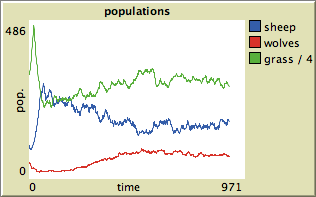
\includegraphics[scale=.666667]{images/wolfsheep/wolfsex_low.png}
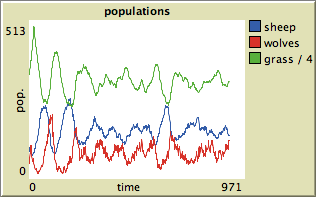
\includegraphics[scale=.666667]{images/wolfsheep/wolfsex_high.png}
\caption{Plot of a Wolf Sheep Predation run with low (left) and high (right) \textit{wolf-reproduce}.}
\label{fig:wsp_wolfsex}
\end{figure}


The configuration space is five-dimensional, making this domain nontrivial to analyze.
The configuration parameters, along with some general observations, are as follows:
\begin{itemize}
   \item \textit{sheep-gain-from-food} -- the amount of energy sheep gain from eating grass.
This parameter has interesting effects on the system.
The effect of changing this parameter from the stable norm is shown in Figure \ref{fig:wsp_sheepfood}.

At lower values, the population of the sheep has difficulty not going extinct.
This almost always results in the wolf population going extinct.

At higher values, sheep live longer and quickly become overpopulated, which causes the grass to become a scarce resource.
With little grass left, the sheep begin to die off.
Once enough sheep have died off, the grass begins to regrow and the sheep begin to reproduce.
This results in sharp increases and decreases in sheep population as the sheep population oscillates between overpopulated and underpopulated.
When the oscillations are of high enough magnitude, the wolves have a high chance of becoming extinct while the sheep population is very low.


   \item \textit{wolf-gain-from-food} -- the amount of energy wolves gain from eating a sheep.
This parameter affects the system in a similar way as \textit{sheep-gain-from-food}.
Lower values cause the wolves to go extinct, while higher values cause more drastic oscillations in wolf and sheep populations.
The effect of changing this parameter from the stable norm is  shown in Figure \ref{fig:wsp_wolffood}.

   \item \textit{sheep-reproduce} -- the percent chance that a sheep will reproduce, per time step.
This parameter has the interesting property that when it is increased, the wolf population increases, but the sheep population remains relatively constant.
When \textit{sheep-reproduce} is too low, the sheep population has difficulties sustaining its numbers, which causes the wolf population to be very low.
The effect of changing this parameter from the stable norm is  shown in Figure \ref{fig:wsp_sheepsex}.

   \item \textit{wolf-reproduce} -- the percent chance that a wolf will reproduce, per time step.
This parameter has relatively little effect on the system, in comparison to the other parameters.
The populations oscillate more when the reproduction rate is higher and more stable with it lower.
The effect of changing this parameter from the stable norm is  shown in Figure \ref{fig:wsp_wolfsex}.

   \item \textit{grass-regrowth-time} -- the amount of time steps a patch of grass takes to regrow.
This is perhaps the strangest behaving configuration parameter.
At higher values, not enough grass grows to sustain a large sheep population, which causes the wolves to go extinct.
At lower values, sheep rarely every die, until they become overpopulated and eat all the grass.
At this point, there is a mass extinction, which causes the wolves to typically go extinct.
In behavior, this parameter is similar to that of \textit{sheep-gain-from-food}.

\end{itemize}
Each of these parameters individually affect the system state.
Even more diverse behaviors can be observed by adjusting several parameters at once.

Several system-level properties have been developed for this domain.
To sample many of these properties and to provide more consistent results, each random configuration is sampled a number of times and averaged.
\begin{itemize}
\item \textit{sheep-extinct?} and \textit{wolves-extinct?} -- the probability that the sheep and wolf populations will reach zero, respectively.

The probability of sheep and wolf extinction is measured by sampling the same configuration numerous times and calculating the percentage of instances they went extinct.
Most often with a specific configuration, the sheep or wolves always go extinct or always do not go extinct.
However, there are borderline configurations in which the sheep or wolves will go extinct while the system is stabilizing into a rhythm.
This metric is useful in distinguishing between these three situations.
Wolves will always go extinct if there are no sheep, but sheep can exist without wolves.
Therefore, the value of \textit{wolves-extinct} is always higher than \textit{sheep-extinct?}.

\item \textit{sheep-average} and \textit{wolf-average} -- the average sheep and wolves given they did not go extinct, respectively.

The average sheep and wolf populations are calculated by averaging the populations at every time step in instances in which they did not go extinct.
Not including extinct populations in the average is important because these instances will introduce significant amounts of bias.
This metric describes how large the population can expected to be.
Along with \textit{sheep-variance} and \textit{wolf-variance}, the averages describes the nature of the population and how it changes.

\item \textit{sheep-variance} and \textit{wolf-variance} -- the variance of the sheep and wolf population over the course of a run.

The variance is calculated with the same data as the average.
This metric describes how much the population changes from time step to time step, since the population is typically rhythmically changing.

\end{itemize}

slp: sheep extinct?, wolf extinct?, average wolf population, average sheep population, variance of sheep population, variance of wolf population

 \subsection{NetLogo Traffic Basic}

config: number-of-cars, acceleration, deceleration

slp: average max speed, average min speed, frequency of traffic jam

 \subsection{Reynolds Boids}

config: num-boids, avoidance, center

slp: density, speed


\section{Forward Mapping Methods}\label{sec:fmalgo}

\begin{itemize}
 \item k-Nearest Neighbor (KNN)
 \item Robust Locally Weighted Regression and Smoothing Scatterplots (LOESS)
 \item ?
\end{itemize}



\section{Experiments}\label{sec:exps}

 \subsection{Forward Mapping}

  \subsubsection{Accuracy}

  \subsubsection{Offline Computation Time}

  \subsubsection{Online Computation Time}

 \subsection{Reverse Mapping}

  \subsubsection{Accuracy vs. Forward Mapping}

  \subsubsection{Accuracy vs. System Run}

  \subsubsection{Offline Computation Time}

  \subsubsection{Online Computation Time}

\cleardoublepage

\chapter{RELATED WORK}
\thispagestyle{plain}

\label{RelatedWork}


\section{Experimentation in ABMs}
\label{sec:abmexp}
Experimental platform for messing around with ABMs: (Bourjot -- ``A platform for the analysis of artificial self-organized systems'' 2004) (relevant?).
Outline 3 tasks for experimentation -- under which conditions expected behavior occurs; validating the system (it works like we planned).
designed a platform
allows the user to experiment with a system with several inputs (analogous to our sampling).
they plot and find the mean behavior of different experiments
they propose that you can use the raw data to compute abstract conclusions about the system.
Suggest using optimization instead of a user.

\fw provides a framework for general experimentation of ABMs.
provides quantitative analysis, instead of qualitative. researchers' qualitative conclusions can be made with the assistance of the quantitative data produced by \fw.

\subsection{Experimentation in Realistic Biological Models}
ABMs have been used to study behaviors in biological systems... Domain specific work interested in system-level behavior: ant lane formation , , fish schools . Most of these studies are qualitative in nature.

marching locusts \cite{buhl2006dom} -- find at which density locusts start swarming, instead of acting as individuals; they note a few SLPs that describe the swarming behavior and show plots that show the relationship between these properties with the density of locusts.
This is an example of manual experimentation, and is something that \fw automates

\cite{couzin2003sol}
models how army ants form lanes.
ants moving to and from the nest.
at low densities, agents come and go randomly.
at higher densities, lanes form that optimize traffic flow.
agent-level property of avoidance turning rate and perception angle of area ahead of the ant.
the authors make a plot that show how ant flow changes with the change of these two parameters.
Also do another experiment where difference in turning rate between incoming and outgoing, shows that higher difference means higher flow.
They make plots and analyze them -- no computer-assistedness.
Other parameters were tweaked to have the system match behavior from videos of real ants.
This was probably done manually.

\cite{parrish2002sof}
Generalized model of fish schooling that aggregate concepts from several previous schooling models.
Fish from a population form into several groups
Measure a number of group-level and population aggregated statistics, such as group size, number of groups, stragglers, collisions, polarization.
Make a number of qualitative conclusions on the effects of agent-level parameters on the system-level properties.
They found that drag and randomness had little effect on fish schooling behavior in comparison to the social forces.
They tested lots of different types of repulsion/attraction curves with different shapes and magnitudes.
With a convex attraction-repulsion curve, stayed closed together and had more collisions. Polarization unaffected.
Changing neighbor scaling to have social forces be weighted based on distance made fish schools smaller and move faster. collisions decreased.

\subsection{Experimentation in Particle Swarm Optimization}

Particle swarm optimization (PSO) is a swarm intelligence technique for finding a solution to optimization problems in a multi-dimensional, continuous search space \cite{kennedy1995pso}.
PSO uses a multitude of agents that ``swarm" around good solutions, hoping to find better solutions.
Agents in PSO are in predetermined neighborhoods in which all members of the same neighborhood share the neighborhood's highest fitness found.
Each agent keeps track of its personal highest fitness found, its neighborhood's highest fitness found and the global highest fitness found.
Then, an agent moves towards each of these maxima with a force of predetermined strength, specified by a parameter provided by the user.
Additional parameters specify the number of agents and how much momentum agents have.
Momentum is defined as how much of the agent's velocity vector in the previous time step is carried into the next time step.

There originally were no guidelines for determining appropriate parameter settings for the following: the number of neighborhoods, the size of the neighborhoods, the constants in the force equation (personal best factor, neighborhood best factor, global best factor, momentum), the maximum speed of the agents, the initial spread of the agents, and the initial velocity.
First, there was an empirical study particle swarm optimization: empirical study \cite{shi1998parameter};
They performed experiments to show how inertia weight (the momentum of a particle) and the maximum speed affect the performance of PSO.
The intuition behind this experiment is that particles that are too fast (i.e., high inertia and high maximum speed) will overshoot optimums, missing them entirely, while particles that are too slow (i.e., low inertia and low maximum speed) will take a long time to reach optimal solutions.
A number of different configurations were used and the results are presented as a table.
There is no way to determine if these parameter values will transfer to other domains other than the experimental one.

more general approach: \cite{van2006study}
provides a more theoretical perspective to particle swarm optimization.
They determine which parameters will cause particles to converge.
They also are able to predict the nature of particle trajectories over time.
However, although this paper provides theoretical results on PSO, the authors explicitly state that the paper is not an approach to determining optimal parameters and points readers to empirical studies like \cite{shi1998parameter}.
\fw can analyze systems such as PSO to find configurations that perform as expected.
This takes the empirical studies one step further than just sampling data points by aggregating information from them.

\section{Prediction of System-Level Behavior}

physics-based control policy \cite{spears2004dpb} -- similar to our approach, but the models are tightly coupled to the domain. the system was designed with system-level models in mind.
Called physicomimetics.
Framework of rules inspired by common physics equations (such as $F=MA$) that can control self-organizing agents.
Agents can form hexagonal lattices, square formations,
Algebraic inversion for inverse mapping is nice. Inspires the nonlinear regression approach in \fw.
For example, in work by Spears et al. \cite{spears2004dpb}, the authors develop a physics-based control policy for
a swarm of mobile robot agents. With this, the swarm-level behavior of the system can be described as a mathematical equation.
System designers of this framework can avoid costly trial-and-error of the controllers by deriving theoretical laws from the controlling functions.
This mathematical analysis of the system is useful and precise, but will
not always extend to other domains. Also, some level of human intuition was required to develop these equations.
Rule abstraction may not develop models that are as accurate as the theoretical behaviors developed by Spears et al., but it will do so
autonomously with methods that can be extended to other domains.

Macroscopic models of swarm robot systems \cite{lerman2002mmf}\cite{lerman2005rpm} -- similar in motivation, but models the system in a more specific way (FSAs). Specific to systems in which agents can be modeled as FSAs. Our approach is more general, since it just looks at parameters.
Describe robots as a stochastic markov process (ie, future state depends only on its present state)
Develop a function $N_x(t)$ -- the average number of robots in state x at time t.
Developed this function as a parametric function, with manual mathematicaly analysis.
Worked on two domains -- collaborative stick pulling and collective object collection.
The $N$ function can be used to describe how the behavior of the robots change over time.
They can also aggregate information about total time spent robots are spending in a sertain state.
The authors plot total time spent in each state in relation to the number of agents.
The plots show that with more agents, the robots spend more time avoiding and less time collecting.
From this, they determine the efficiency of how each robot is affected by group size.
This work develops a model of how long the collection task takes, given the number of robots.
They developed functions that describe the space, which is what we are doing.
this is domain-dependent, as the mathematical analysis will change for different systems.
Also, this is not applicable to many ABMs that would be difficult to model the individual agents as sMDPs.
\fw differs from this in two major ways. First, the authors do not discuss how inverted analysis could be applied:
that is, given a value for the macroscopic behavior, generate parameters for a swarm with that property. However,
this was probably not an explicit goal of their work.
Second, the way the authors model agents is more restrictive than the model used in rule abstraction. Some swarm systems,
such as boid flocks, behave based on a sum of forces, not as FSAs. Therefore, Lerman et al.'s work may not be able to intuitively
model such a system. Meanwhile, rule abstraction's view of an agent can represent an FSA:
the parameters in a rule abstraction would include properties of each state of the FSA as well as transition probabilities.
Therefore, I believe that rule abstraction is more general than the work by Lerman et al. and will be applicable in more domains.


Use evolutionary search to look for nonconvergence in the NetLogo Flocking and V-Formation Flocking domains \cite{stonedahl}
Use genetic algorithms to search the configration space for system-level properties of interest.
Find a system that converges as fast as possible.
Make a quantitative measure of the property (like we do with SLPs).
Main difference: optimization vs. a goal, while I am just fitting a specific desire.
Plots the results as a set of boxplots that show the ranges of configurations that generate converging behaviors.
The correlations between the configuration parameters are mostly ignored in these plots, but they do show the ranges of behaviors that produce desired behavior.
They showed that genetic algorithms outperform hill climbers and random search with the same number of model runs.
This approach is similar in many ways: it is using optimization to make a sort of reverse mapping.
It is domain independent, given that the user defines the quantifiable behavior.
However, it uses optimization, which requires online time, to find results.
I develop a prelearned mapping which is fast to query and saveable for later use.

%not entirely relevant -- Idea of system-level control.... robot swarms \cite{mclurkin2004srt} -- tightly coupled with domain, describes the behaviors as actions (not properties), splits behaviors into hierarchies.


\section{Inversion of Forward Mappings}
Approaching the reverse-mapping problem has been tackled before by inverting the forward mapping.
The idea is not new, but the idea of returning a functional approximation of the reverse space is new.
All of these approaches return a single solution, instead of a space.
Also, many of these approaches are iterative and online.

One of the first approaches is to simply directly learn the reverse mapping as a supervised learning problem\cite{widrow1985adaptive}.
This doesn't work because if the forward mapping is many-to-one, this is trying to learn a one-to-many relationships, which is bad.
The reason this is bad is called the ``convexity problem", where if set of all possible solutions is not convex, the average of some values from it may not be within the solution space, yielding bad results. \cite{jordan-forward}.

Work has been done in inverting multilayer neural networks.
All of these are optimization techniques.
They do not return an actual mapping.
Also, the techniques are restricted to neural networks (and are thus not algorithm-independent).

\begin{itemize}
\item (A Linden and J Kindermann ``Inversion of multilayer nets'' 1989 -- optimization problem solved by gradient descent) Minimize $\sum (Y_i - f(X_i))^2$ \cite{linden1989inversion}
\item (Bao-Liang Lu ``Inverting Feedforward Neural Networks using Linear and Nonlinear programming'' 1990 --  Authors mention the problem of the inverse problem being ill-posed because the mapping is one-to-many .formulate the inverse problem as a nonlinear programming problem (constrained optimization problem), a separable programming problem or a linear programming problem). Uses a modified simplex method for solving linear programming problems.
Ability to specify exterior constraints.
Various points can be derivd by setting different constraint functions. \cite{lu1999inverting}
\item (Michael I. Jordan work with robot arm ``Forward Models: supervised learning with a distal teacher'' -- asks the question, what configuration of the robot arm will yield this behavior?)
returns an individual solution.
no way to tell which of the infinite solutions will be returned.
\end{itemize}

(S. Lee and R.M. Kill ``Inverse Mapping of continuous functions using local and global information'' 1989 -- iterative update towards a good solution)
Iterative approach to approximating any continuous function.
It incrementally approaches a good solution, and leaves local minima to continue searching for more solutions.
One requirement, however, is the Jacobian must be calculated (or approximated), which makes this approach difficult to apply to some functions, such as piecewise or discontinuous ones.
The authors suggest their approach would work well with neural networks, as the jacobian for them is easy to compute.
Also, it just returns one solution.



\section{Multilinear Interpolation}
\label{sec:multilinear}

  % Multilinear Interpolation
    % Concept - given corner points of a hypercube (knots), interpolate some point inside of it with linear interpolation; interpolate dimension my dimension until the point is reached.
Multilinear interpolation is a dynamic approach that uses multi-dimensional interpolation between ``knots" to generate a smooth surface across a space of any dimension \cite{davies1997multidimensional}.
Knots are sampled data points, scattered across the behavior space in a regular fashion such that the knots, when connected, form hypercubes.
When a point $\mathbf x$ is queried, multidimensional interpolation is performed using the corners of the hypercube to infer the value of $\hat y$.

Multilinear interpolation serves as an inspiration for my simplical complex inversion approach.
They are practically identical, except that SCI segregates the space into simplexs, instead of hypercubes.
This modification was necessary because intersections can be found at the edges of simplexes and connected with line segments.
Slices through a gradient in a hypercube that represent a particular value are not linear.
Therefore, the representation is more complicated and makes working with them more difficult.
Working with: finding intersections (combining reverse mappings), defining a piecewise curve that represents a SLP can be done with just points, instead of curves.
SCI is therefore less smooth because of the linearity of the pieces, but easier to work with.

    % Downside - sampling needs to be systematic: remedy- use another regression algorithm to build the knots. This has the benefit of being faster than other approaches (the interpolation is fast, the regression may be slow, and the knots can be built ahead of time)
A major downside to standard multilinear interpolation is that the sampling needs to be systematic and evenly spaced.
To remedy this situation, another regression algorithm can be used to compile a set of evenlyspaced points.
SCI uses this approach so that it can use randomly sampled data.
These evenly spaced inferred points are then passed to a traditional multilinear interpolation approach.

    % Faster than some of its counterparts
    % builds smooth mappings of multi-dimensional spaces





\cleardoublepage

\chapter{CONCLUSIONS AND FUTURE WORK}
\thispagestyle{plain}

\label{Conclusions}

In the course of this dissertation, I have outlined the inner workings of the \framework.
The requirements and strategies for defining system-level properties were enumerated in Chapter \ref{Defining}.
The approach that \fw takes in solving the forward-mapping problem with regression was explained in Chapter \ref{ForwardMapping} and proven accurate and efficient in Chapter \ref{Results}.
Formulating the problem of prediction  system-level properties of an ABM as a regression problem leads to effecive prediction mechanisms.
The approach that \fw takes in solving the reverse-mapping problem with the novel simplical complex approach was explained in Chapter \ref{ReverseMapping} and proven accurate and efficient in most cases in Chapter \ref{Results}.
Inverting an approximation of the forward mapping proved to be an accurate and general way to build a reverse mapping to solve the reverse-mapping problem.

% The research project reached its aims
   % what did I try to achieve?
      % The main goal of the \framework is to bridge the gap between agent-level parameters and system-level properties.
The main goal of the \framework was to bridge the intuition gap between agent-level configuration parameters and system-level property values.
The forward mapping can be used by researchers to perform experimentation and is much faster than interacting with the ABM directly.
Whether the researcher is currently using an optimization approach or manually inspecting the system, using the forward mapping is  more convenient and faster than interacting with the ABM directly.
Only a small amount of error is incurred by using \fw, which is greatly outweighed by the benefits.
The reverse mapping can be used as a replacement for optimization and to provide the space of configurations that will satisfy a system-level property, which is useful for finding a number of configurations that will generate desired behavior in an ABM.
Also, researchers can use the reverse mapping as an aid to making qualitative conclusions about the nature of the system-level properties.

In Chapter \ref{Framework}, the following constraints were placed upon the implementation of \fw:
\begin{itemize}
      \item Domain-independent: The design of \fw should minimize the amount of configuration that is needed for each new domain;
      \item Algorithm-independent: any regression algorithm should be able to be applied with \fw;
      \item Accurate: \fw should generate accurate predictions and control suggestions; and
      \item Fast for the user: interactions with the models generated by \fw should require minimal computational time.
\end{itemize}

\fw achieved these goals. None of the four domains that \fw was applied required special modifications to the implementation of the framework in order to function correctly.
The same interfaces were used for each domain, and can be used for future domains.
The reverse-mapping solution simplical complex inversion is algorithm-independent, as shown by the fact that the core framework did not have to be modified in order to accommodate k-nearest neighbor, LOESS, or non-linear regression.
Future regression algorithms could be used for the forward mapping and the reverse mapping would require no changes.
Therefore, \fw is domain- and algorithm-independent.

The results in Chapter \ref{Results} show that the implementation of \fw produces accurate results across all of the domains that were tested.
In most cases, \fw was fast for the user.
From the results, forward mapping queries are thousands of times faster than actually querying the ABM.
This is important for researchers who wish to experiment with ABMs, but do not wish to spend upwards of eight seconds for each sample.
A query to the reverse mapping is typically lsss than two seconds; however, the response time does not scale well with dimensionality.
With higher dimensions, the reverse mapping is not fast for the user, and optimization or analyzing sub-portions of the configuration space should be considered as alternatives.
Therefore, \fw is accurate and efficient when dealing with low-dimensional behavior spaces.

In conclusion, the results show that \fw satisfies many of these constraints and satisfies the major goal of bridging the intuitive gap between agent-level configuration parameters and system-level property values.

\section{Future Work}

In the course of the research, a number of possible directions for future work have arisen.
Each of the following subsections discuss a possible subproblem in ABM meta-modeling or extensions to \fw that could produce interesting results.

\section{Extension: Specifying Ranges for System-level Properties}
\label{sec:ranges}

One of the major problems with SCI is that queries can easily become overspecified.
This is the case if the number of system-level properties exceeds the number of configuration parameters.
In the case of overspecification, the reverse mapping will not return any solutions, since they do not exist.
To avoid this problem, SCI could be altered to take as input \textit{ranges} of system-level property values, instead of specific values.
This would provide some leeway and allows for more possibility of intersections.
Instead of the solution of the reverse-mapping query being a hyperplane, it would become a hyperspace.
The query plane used to intersect with the reverse mapping would also be a hyperspace, bounded by two hyperplanes.

This extension would complicate the implementation significantly.
In order to implement this extension in SCI, the equations used would be inequalities, complicating the calculation of the intersection.
Any point that is satisfied by the set of inequalities over all simplexes could satisfy the system-level property ranges.
In the rest of this subsection, the QT approach is described, but the implementation is left as future work.

The Quad-Tree (QT) approach for inverting the forward mapping is intended to be simpler to implement than SCI.
Also, specifying ranges for system-level properties is more natural in QT than in SCI.
QT performs the same tasks as SCI, but instead returns a set of subspaces that must or could possibly contain configurations that satisfy the desired system-level property configuration.
In general, a quad-tree is a tree data structure in which each node either has zero or four children.
A quad-tree can be used to iteratively segregate a two-dimensional space into several subspaces in order to give certain portions of the space more detail.
Quad-trees use a notion of ``black," ``gray," and ``white" cells: black cells represent a subspace in which all values are black, white cells represent a subspace in which all values are white; and gray cells represent a subspace in which some values are white and some values are black.
The benefit of using a quad-tree structure is that black and white cells do not need to be expanded, as all of their values are already determined.
However, gray cells are broken down further by segregating its space into four children, which may be black, gray, or white.
Grey cells can be broken down as many times as desired, but typically, quad-trees are capped at a certain depth, which I call the ``granularity depth."

The idea of quad-trees can be used in the reverse mapping to approximate the solution space.
Black nodes are ones in which all values within the subspace match the query;
white nodes are ones in which none of the values within the subspace match the query;
and gray nodes are ones in which some of the values within the subspace match the query.
Instead of using squares to split the subspaces, QT must use hypercubes, since the configuration space is typically not two-dimensional.
QT returns all the gray cells and black cells found by this approach as an answer to a user's query.

Gray nodes are broken down iteratively until the granularity depth is reached.
QT breaks down a hypercube (a pair of simplexes) by querying the forward mapping for the points needed to break a single $n$-dimensional hypercube into $2^n$ hypercubes (split a line into two lines, a square into four squares, a cube into eight cubes, etc.).
Each new hypercube is then evaluated to see whether it contains the desired system-level property values or not, which can be determined by comparing the desired system-level property with the observed maximum and minimum among the corners of each hypercube.
If the desired system-level property value is less than the maximum, and greater than the minimum, then possibly an intersection satisfying all system-level properties exists within this hypercube.
If one of the values is not contained within this range, then the hypercube is marked as ``white" and does not need to be expanded further.

This approach has the benefit that the intersections of hyperplanes do not need to be calculated, which may be difficult to implement.
Although it is less accurate and the space it returns is not continuous, it serves the purpose of the reverse mapping in many ways.
It still returns configurations that the user should use to generate the behavior and can still be visualized to show the nature of the configurations that generate a particular system-level property.

Another motivation for using QT over SCI is that specifying ranges for system-level properties is difficult to represent in SCI because all of the equations are inequalities.
Meanwhile, the implementation in QT is quite simple because hypercubes either do or do not contain the target values.
Details on the uses of ranges in querying the reverse mapping are discussed in Section \ref{sec:ranges}.

\begin{figure}[ht]
\centering
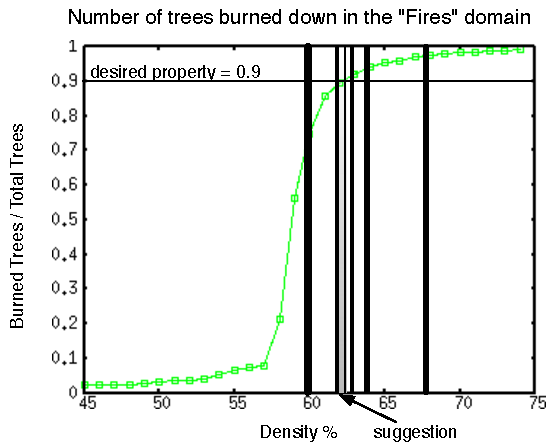
\includegraphics[scale=1]{images/QTfires.pdf}
\caption{The subspaces generated by QT represent a range of configurations that are close to satisfying the desired system-level property.}
\label{fig:qtfires}
\end{figure}

The usage of QT on the fires domain is visualized in Figure \ref{fig:qtfires}.
The thicker bars represent earlier subdivisions.
First, the space was split into the ranges 45--60 and 60--75.
The system-level property ranges from .02 to .7 in the 45--60 subspace, so this space can be ignored in future divisions because it does not contain the value .9.
The other half is subdivided at 67.5.
This process continues five times, which is the granularity depth in this case.
In a situation in which several solutions are possible, several subspaces will be returned as candidate configuration spaces.


\begin{figure}[ht]
\centering
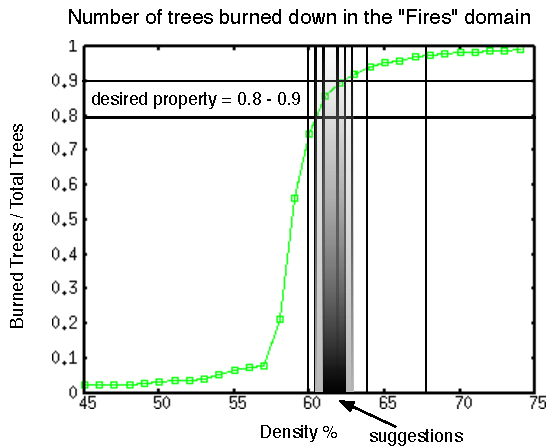
\includegraphics[scale=1]{images/QTfiresranges.pdf}
\caption{The subspaces generated by QT represent a range of configurations that are close to satisfying ranges of the desired system-level property.}
\label{fig:qtfiresranges}
\end{figure}
To handle ranges of system-level property values, only minor modifications to QT must be done.
The space is subdivided in the same way as standard QT; however, spaces that lie entirely within the ranged are marked as ``black" and do not need to be subdivided further.
Ranges marked as ``white" do not need to be subdivided either.
Gray areas are inspected more closely in order to increase the detail of the reverse mapping solution.
A set of configuration spaces is returned, representing the configurations that will satisfy the system-level property range.
This process is visualized in Figure \ref{fig:qtfiresranges}.



The caveat with this approach is that in non-monotonically changing domains, the maximum and minimum values at the corners do not necessary accurately describe the maximum and minimum within the hypercube.
If there exists a local minima or local maxima within a cube, the feature will be ignored.
To avoid this problem, the starting grid of hypercubes should be sufficiently detailed.



\subsection{Extension: Adaptive Meta-models}

In some agent-based models, a hidden property may change over the course of several runs, or perhaps within a same run, over time.
A hidden property is a feature of the environment that changes the behavior of the agents in some way, but is not directly detectable.
In the case that the hidden property does not change, the learned mappings will adapt to this hidden variable and the mappings will continue to be accurate.
However, in cases in which the hidden property changes over time, the learned mappings must be adaptive, since the value of the hidden property is not part of the configuration vector.
Because of a changing hidden property, the system-level behavior of a system can change, yet still be running the same configuration.

Wind in a flocking ABM serves as a good example of this phenomena.
A strong wind can change the behavior of a flocking system to be less cohesive.
However, the value of the wind is not predictable, which can cause predictions about the system to be erroneous.

To tackle this problem, the meta-models built by the forward and reverse mapping must be adaptive to the current conditions in the ABM.
I propose an online optimization technique that incrementally adjusts the behavior of the system to compensate for hidden changes in the system.
A continuous stream of current system-level property values will be provided as inputs into the framework.
The forward mapping will predict what should be happening with this configuration; this prediction would be compared to the actual system-level behavior.
The distance between the predicted and actual would be minimized by incrementally adjusting (i.e., hillclimbing or optimization) the configuration in order to minimize this gap.
Over time, the difference between the predicted and actual value will converge to zero.

The approach described here is an optimization approach, but is different from standard optimization because the initial starting position provided by the forward mapping is presumably close to the optimal configuration.
Also, the derivative of the mapping can be used in a gradient ascent approach, in which the derivative is calculated from the forward mapping.
Hidden variables typically will not change the nature of the system, only the specific values.
That is, increasing one configuration parameter is likely to have the same sort of effect regardless of hidden parameters, but not exactly.


% hidden properties that can change

\subsection{Correlated System-level Properties}
% need to predict all system-level properties as one.

One of the major assumptions used in the \fw approach to learning the reverse mapping is that the system-level property values are not correlated.
This assumption allows the reverse mapping problem to be split into a number of reverse mapping subproblems (one per system-level property).
However, if the properties are correlated, the result of the reverse mapping may be inaccurate.

For example, consider two system-level properties $a$ and $b$ are correlated such that $a \cdot b^2 = 1$.
Suppose that \fw, while solving the reverse-mapping problem, averages $a$ and $b$ separately for the following two instances: $a=100, b=\frac{1}{10}$ and $a=400, b=\frac{1}{20}$.
The averages are $a=250, b=\frac{1}{15}$; however, $250 \cdot \frac{1}{15} \neq 1$, which clearly is not a valid instance.

To avoid this problem, a multi-variate learning approach must be taken.
The forward mapping must be learned with a multi-variate regression algorithm, which must then be inverted in a multi-variate manner, as well.
This type of approach could consider all properties at once, and would therefore be immune to this problem.



\subsection{Handling Many Dimensions in Simplical Complex Inversion}

In Chapter \ref{Results}, the five-dimensional configuration space of the Wolf Sheep domain proved to be too large for simplical complex inversion.
I have considered a few approaches to tacking this problem in future work.

The first option is to use optimization instead of building a mapping.
This approach has the major problem that it will not return a space of solutions---it will only return one.
In many situations, this will be acceptable if the user is attempting to find a satisfactory configuration that will generate a specific system-level behavior.
An interesting point to note is that the behavior spaces are typically continuous.
Therefore, if there are many configurations that will satisfy the particular system-level property specification, they will probably exist near the point found with optimization.
A hillclimbing approach will move along these ridges of equal fitness and could return several possible configuration points.
This will work particularly well in situations in which the solution configuration space is linear, because the optimization simply follows a line.
However, with higher-dimensional configuration solution spaces, the representation of a hyperplanar solution space would be difficult to develop. 

Another approach to the problem would be to dynamically generate the majority of the simplical complex at run time.
This approach would allow a smaller portion of the mapping to reside in memory, making this problem far more tractable.
A specific simplex can contains a desired system-level property if the system-level property is within the minimum and maximum values of the simplex's corners.
These candidates can be broken up further to generate a more accurate mapping of the configuration solution space.
The major difficulty in this approach is the existence of local minima and local maxima within a simplex.
Consider the following example: a simplex has a minimum system-level property value of 4 and a maximum system-level property value of 6.
The value being sought is 7.
It is quite possible that at some point in the forward mapping, the value of the system-level property reaches 8, then decreases back down to 7 at the edge of the simplex.
It is impossible to determine that this is the case from just the values of the simplex corners.
One way in which a local maxima (or minima) could be inferred to exist within a simplex is to approximate the derivative (i.e., rate of change) of the system-level property at the edges of the simplex.
For example, if at all edges, the system-level property is increasing, then it is highly likely that a system-level property local maximum exists within this simplex.
The derivative can be approximated by viewing the values of other knots nearby, or by sampling additional points to approximate the derivative.
The domains I sampled and many of the domains discussed in Chapter \ref{RelatedWork} do not exhibit behavior spaces with many local minima and maxima.
Typically, the system-level property increases monotonically or has a single maximum, as the configuration changes.
Therefore, the simplex-based approach in approximating the derivative would likely be successful, since there are typically  only a limited number of maximums.

Although many approaches can be applied to reduce the computational complexity of solving the reverse problem, most approaches will suffer the curse of dimensionality, as does SCI.
As more dimensions are added, optimization techniques will have to search more of the space and SCI-type approaches will require more subspaces.
Even approaches similar to non-linear regression, which can be functionally inverted, become more complex with more dimensions.
With NLR, more model parameters and more variables make the system of equations significantly more difficult to solve.
Regardless of scaling issues, any improvement of performance in solving the reverse-mapping problem will allow researchers to inspect and analyze more complex agent-based models.

\subsection{Optimization of a System-Level Property}

In some cases, researchers may not want a configuration that produces a specific system-level behavior, but instead produces ``the best" system-level behavior.
In this case, an optimization approach, similar to that in work by Stonedahl and Wilensky (2010)\nocite{stonedahl}, could be used to find an optimal behavior.
A SCI-type approach would not be needed, because typically an ``optimal" behavior will be a single point, and does not necessarily need to be represented as a hyperplane.

Using the forward mapping could greatly improve the performance of work similar to that of Stonedahl and Wilensky, since instead of interacting with the ABM directly to calculate the fitness function, the optimization algorithm would be interacting with the forward mapping.
This method would greatly reduce the computation time of a particular optimization, at the cost of spending a significant amount of time training the forward mapping.
If many optimizations are to be performed, training the forward mapping would save time in the long run, since it can be used as many times as needed.
Instead, in a traditional optimization approach, the ABM would have to be re-sampled every time, even if the space being searched is the same as previous search spaces.


\section{Closing Thoughts}

It is my hope that this dissertation will spur additional research projects and discussions in tackling the problem of more efficient experimentation and deeper analysis of agent-based models.
This dissertation not only served to document for my particular approach and implementation, but also defined a number of core problems in this field.
Many alternative implementations are possible, some of which have been outlined in the Future Work section of this chapter.
Researching these additional solutions  will  lead to the discovery of new advances in the analysis of agent-based models.
Additional tools and theory regarding analysis of agent-based models will improve their usefulness in current models and their applicability to newer, more complex systems.



\cleardoublepage

%\appendix

%\chapter{User Guide for the \fw Software}
\thispagestyle{plain}


\section{Regression Plug-In Interface}
\label{RegressionInterface}

I will explicitely detail the interface that a regression algorithm to be plugged into \fw needs to have.


%\cleardoublepage


%\chapter{Code Samples}
\thispagestyle{plain}

\label{CodeSamples}

A bunch of code samples will be put here. These will serve as examples to show how to do things or to show how easy they are

\section{Sample Java/NetLogo Sampling Program}
\label{SamplingProgram}

This code example will show how to write a sampler for \fw.





%\cleardoublepage



\thispagestyle{plain}
\bibliographystyle{aaai}
\bibliography{thesis}

\end{document}
